%----------------------------------------------------------------------------------------
%	PACKAGES AND OTHER DOCUMENT CONFIGURATIONS
%----------------------------------------------------------------------------------------

\documentclass[11pt, twoside, openright]{report}

\usepackage[T1]{fontenc}
\usepackage{titlesec, blindtext, color}
\usepackage{pdflscape}
\usepackage{graphicx}
\usepackage[utf8]{inputenc}
\usepackage{ragged2e} 
\usepackage{mathpazo}
\usepackage[a4paper, total={6in, 8in}]{geometry}
\usepackage{lscape}
\usepackage{float} 
\usepackage{enumitem}
\usepackage{fancyhdr}
\usepackage{caption}
\usepackage[dvipsnames]{xcolor}
\usepackage{hyperref}
\usepackage{dirtree}
\usepackage{listings}
\usepackage{booktabs}
\usepackage{amssymb}
\usepackage{makecell}
\usepackage{rotating}
\usepackage{appendix}
\usepackage{pdfpages}
\usepackage{epigraph}
\usepackage[htt]{hyphenat}

\definecolor{gray75}{gray}{0.75}
\titleformat{\chapter}[hang]{\Huge\bfseries}{\thechapter\hsp\textcolor{gray75}{|}\hsp}{0pt}{\Huge\bfseries}
\setlist[description]{leftmargin=\parindent,labelindent=\parindent}
\epigraphsize{\small\itshape}
\setlength\epigraphwidth{8cm}
\setlength\epigraphrule{0pt}

% New commands
\newcommand{\hsp}{\hspace{20pt}}
\newcommand{\blankpage}{\mbox{}\thispagestyle{empty}\clearpage}
\newcommand{\question}[1]{\begin{description} \item[Q.] \textbf{#1} \end{description}}
\newcommand{\answer}[1]{\begin{description} \item[A.] #1 \end{description} \bigbreak \bigbreak}

% New environments
\newenvironment{titlemize}[1]{%
  \paragraph{#1}
  \begin{itemize}}
  {\end{itemize}}
\newenvironment{myepigraph}[3]{\epigraph{\textit{``#1"}}{--- \textup{#2}, #3}}

\makeindex
 
\lstset{
  basicstyle=\ttfamily\footnotesize,
  breakatwhitespace=true,           
  breaklines=true,
  captionpos=b,
  commentstyle=\color{gray},
  frame=single,
  keepspaces=true,
  keywordstyle=\color{blue},
  linewidth=0.95\textwidth,
  numberstyle=\tiny\color{gray}, 
  rulecolor=\color{black},           
  showspaces=false,                 
  showstringspaces=false,          
  showtabs=false,                  
  stepnumber=1,                     
  stringstyle=\color{Green},      
  tabsize=2,	                     
  xleftmargin=0.05\textwidth        
}  
%--------------- DOCUMENT --------------
\begin{document}
%--------------- TITLEPAGE --------------
%------------------------------------------------------
%	TITLE PAGE
%------------------------------------------------------

\begin{titlepage}
\newcommand{\HRule}{\rule{\linewidth}{0.5mm}}
\center

%------------------------------------------------
%	Headings
%------------------------------------------------

\textsc{\LARGE MSc in Computer Science }\\[1.5cm]
\textsc{\Large Information Systems Design}\\[0.5cm]

%------------------------------------------------
%	Title
%------------------------------------------------

\HRule\\[0.4cm]

{\huge\bfseries OS Project Study -- Chromium}\\[0.4cm]

\HRule\\[1.5cm]

%------------------------------------------------
%	Author(s)
%------------------------------------------------

\begin{minipage}{0.4\textwidth}
	\begin{flushleft}
		\large
		\textit{Alumni:}\\
		Garea Cidre, \textsc{Javier}\\
		Sande Costa, \textsc{Martín}
	\end{flushleft}
\end{minipage}
~
\begin{minipage}{0.4\textwidth}
	\begin{flushright}
		\large
		\textit{Supervisor:}\\
		Sánchez Penas, \textsc{Juan José}\\
	\end{flushright}
\end{minipage}

%------------------------------------------------
%	Date
%------------------------------------------------

\vfill\vfill\vfill

{\large January 23, 2020}

%------------------------------------------------
%	Logo
%------------------------------------------------

\vfill\vfill

\includegraphics[width=0.5\textwidth]{img/logoudc.png}\\[1cm]
%------------------------------------------------------------
\vfill
\end{titlepage}
\newpage
%--------------- INDEX --------------
\blankpage
\addtocontents{toc}{\vspace{-1cm}}
\pagenumbering{roman}
\setcounter{page}{1}
\tableofcontents
\newpage
\blankpage
\pagenumbering{arabic}
\setcounter{page}{1}
% -----------------------BODY----------------------
\chapter{Introduction}

\section{Introduction to Chromium project}
Following the Chromium Project official website \cite{chromium}, \textit{``Chromium is an open-source browser project that aims to build a safer, faster, and more stable way for all Internet users to experience the web"}. This project is the Open Source version of one of the most popular web browser nowadays, Google Chrome.

Chromium was released under a BSD license on 2008 \cite{release} by Google, at the same time that Chrome did. The purpose of the project was to distribute the source code of the Chrome browser, in order to enable third-party developers to study, modify, extend, and redistribute it. For the time being, following OpenHub charts, this project has more than 25 MLOC \footnote{Million Lines Of Code} and more than 9,000 commits per month. This commits are not only made by Google but for different organizations and independent developers. 

Even that this project integrates more than 30 languages, near the 50\% of the code is written in \texttt{C++}.


\section{Relationship with Google Chrome}

Although Chrome has more features than Chromium, Chromium provides the vast majority of source code for Google Chrome, including the user interface, the Blink rendering engine, and the V8 JavaScript engine. Thus Google chose the ``Chromium" name as an analogy of chromium metal forged into chrome plating.
\begin{figure}[H]
    \centering
    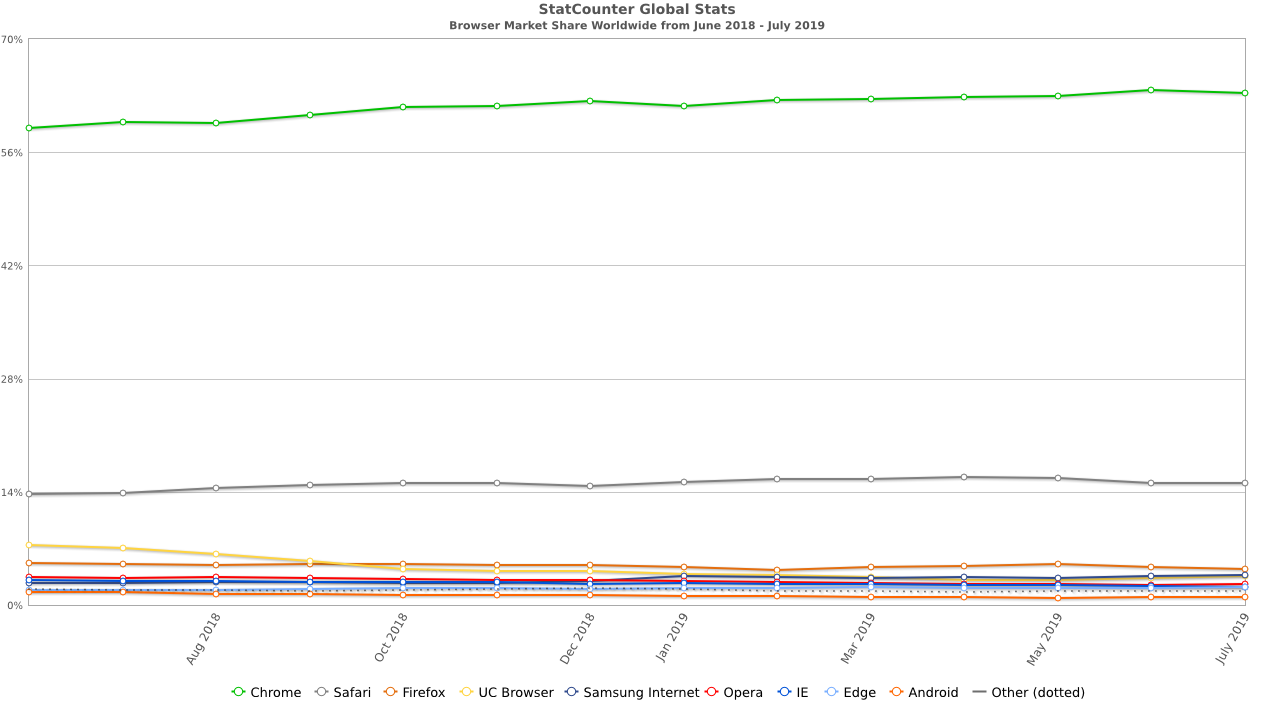
\includegraphics[width=\textwidth]{img/compare.png}
    \caption{Browser usage as of 2019}
    \label{fig:usage}
\end{figure}
As of 2019, StatCounter \cite{usage} (figure \ref{fig:usage}) estimates that Chrome has a 63\% worldwide browser market share across all platforms.


\section{Assignment goals}
The two main goals of the assignment are:

\begin{enumerate}
    \item Applying and contrasting all the knowledge acquired during the theoretical lectures and the invited talks to the study of a real, professional, complex open source project.
    \item Producing a report summarizing all the findings and derived proposals (i.e., this document).
\end{enumerate}


\section{Document structure}
From now on, this document is structured as follows:
\begin{description}
    \item[Chapter \ref{chap:methodology}] Aims to introduce the contribution policy and the technological tools used in the project.
    \item[Chapter \ref{chap:architecture}] We describe some technical aspects about Chromium's software architecture, delving in its multi-process characterization.
    \item[Chapter \ref{chap:design}] The IPC Component is analyzed and described. We also elaborated a set of UML diagrams that helped us to detect some software Design Patterns.
    \item[Chapter \ref{chap:quality}] The key concepts of quality are studied over the project in this chapter.
    \item[Chapter \ref{chap:accessibility}] We take a view on the main accessibility features of Chromium.
    \item[Chapter \ref{chap:interview}] A short but valuable interview with Julie Jeongeun Kim, a Chromium's developer, is presented.
    \item[Chapter \ref{chap:conclusions}] This essay ends with a short impression about what we learned during the analysis and discuss the possible lines of future work.
\end{description}
\chapter{Development methodology and tools}
\label{chap:methodology}

This chapter aims to introduce the contribution policy and the necessary tools to contribute to the Chromium project.


\section{Development methodology}
Chromium is an open source software project with a specific contribution policy. This is detailed in its official documentation in several sections \cite{contributing,lifeofchromedev,contributingguide}.

The first important detail of the project is that it includes other projects such as v8 \cite{v8} that have their own workflow and, therefore, to contribute to these sections we must review the corresponding documentation. In this case we will focus on the general lines of the Chromium workflow.

The pipeline (figure \ref{fig:contributing_pipeline}) that allows a developer to contribute code to the project goes through: developing the code, creating a change and build it, testing the code, uploading the change for a review and finally committing the patch. If all stages are successfully passed, a satisfactory contribution will have been made.

\begin{figure}
    \centering
    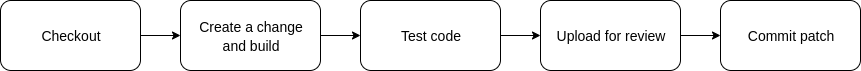
\includegraphics[width=\textwidth]{img/contributing_pipeline.png}
    \caption{Chromium's contributing pipeline.}
    \label{fig:contributing_pipeline}
\end{figure}

\subsection{Initial considerations}

Before delving into details of the contribution pipeline we must pay attention to certain details.

To contribute to the project it is necessary to accept the Contributor License Agreement, which can be individual or corporate depending on the type of contributor. If it is the first contribution, the patch must include a modification of the \texttt{AUTHORS} file so that it includes the name and contact information of the individual or organization that contributes.

It is also important to keep in mind that there is a discussion group as well as various methods to contact developers and code reviewers. It is highly recommended to contact them before getting to work to introduce a new feature or fix a bug.

\subsection{Code checkout}

Chromium is a very large project \footnote{Only the executable file weighs approximately 1.3GB in Linux Debug.}, So we need a slightly powerful machine to work with. To get an idea of the type of machine needed, the documentation indicates that we need a 64-bit machine, even if we are going to build a 32-bit executable, since linking requires more than 4GB of RAM. It is also recommended that the machine has many cores, lots of RAM and a second hard drive for the source code and the building.

If we have that machine, we can proceed to download the source code. The process varies between platforms, but can be summarized in two main points:
\begin{itemize}
    \item Install Depot Tools, a collection of dev utilities.
    \item Run \texttt{fetch chromium} to get all the code and generate the build files.
\end{itemize}

Keep in mind that in order to build in Android it is needed a Linux environment and for iOS it is needed a Mac environment.

\subsubsection{Depot Tools}

Depot Tools is a set of scripts/utilities that:
\begin{itemize}
    \item Manage all checkouts in the Chromium source tree.
    \item Generate the build files for your platform.
    \item Upload your changes to Gerrit \footnote{Used app for the code review process.} for review.
\end{itemize}

\noindent The main utilities for the project are gclient and git-cl.
\begin{description}
\item[gclient] Syncs the source tree and creates build files for your platform.
\item[git-cl] Manages the integration with code review and tryjobs.
\end{description}

\subsection{Modifying and Commiting}

If we have chosen a change to work on, and have discussed it with a senior, we can proceed to follow the Commit Checklist of the project \cite{checklist}.

At the time of writing this document, the checklist steps are:
\begin{enumerate}
    \item \textbf{Create a new branch.} Before starting any development work, it's necessary to create a new branch.
    \item \textbf{Make your changes.} It is important to follow the project code style guide \cite{style_guide}. If the change is going to have a large impact on Chromium it requires a design doc. This design doc has is own review process.
    \item \textbf{Make sure the code builds correctly.} After coding changes, it is necessary to check that common targets build correctly. Note that it's easy to inadvertently break one of the other builds you're not currently working on without realizing it.
    \item \textbf{Test your changes.} For obvious reasons, the code has to be tested. Make sure you cover all code paths you changed.
    \item \textbf{Write unit or browser tests for any new code.} It is recommended to automate every manual test did in the previous stage.
    \item \textbf{Ensure the code is formatted nicely.} Official documentation specifies the \texttt{git cl format {-}{-}js} command \footnote{\texttt{{-}{-}js} option stands for JavaScript supporting.} in order to run the clang auto formatting tools.
    \item \textbf{Check over your changes.} As in the previous stage, the documentation indicates the \texttt{git upstream-diff} in order to check the changes from the most recent checkpoint on the remote repository.
    \item \textbf{Stage relevant files for commit.} Since the project uses git, the relevant files have to be staged for commit using the \texttt{git add} command.
    \item \textbf{Commit your changes.} Use the \texttt{git commit} command. Note that documentation provides some tips for writing proper commit messages.
    \item \textbf{Squash your commits.} When there are a lot of commits made, it is useful to squash the commits in a single commit in order to avoid commit-by-commit merge conflicts.
    \item \textbf{Rebase your local repository.} After commiting, local branches have to be updated with remote changes that have landed since the beginning of the development work. It is also necessary to delete any branch that match the remote repository. This is done by the \texttt{git rebase-update} command. The process can lead into rebase merge conflicts, which should be manually fixed. Since rebasing has the potential to break builds, it is recommended to try re-building after the process.
    \item \textbf{Upload the CL to Gerrit.} This can be done with the \texttt{git cl upload} command.
    \item \textbf{Check the CL again in Gerrit.} The \texttt{git cl web} command takes you to the Gerrit URL associated with the current branch. Here you can check and verify that the uploaded files are correct.
    \item \textbf{Make sure all auto-regression tests pass.} Click \texttt{CQ dry run} and fix any errors. Otherwise the CL won't pass the commit queue (CQ) checks. It is recommended to wait until the CQ Dry run pass before notifying the reviewers since the results may require major changes.
    \item \textbf{Add reviewers to review your code.} There are two ways to do this: you can click \texttt{Find Owners} or run the \texttt{git cl owners} command. Each file with changes in the CL has to be approved by an owner unless you are one of them for some files.
    \item \textbf{Implement feedback from your reviewers.} Reply to all comments from the reviewers on Gerrit and mark all resolved issues as resolved clicking \texttt{Done} or \texttt{Ack}. Click \texttt{Reply} when your CL is ready in order to notify your reviewers that your CL is ready for review again.
    \item \textbf{Land your CL.} Once you have obtained a Code-Review+1 on Gerrit, from at least one owner for each file \footnote{It may be helpful to wait for all your reviewers.}, you are able to land your changes. Click \texttt{Submit to CQ} to try your change in the commit queue (CQ), which will land it if successful.
    \item \textbf{Cleanup.} Run \texttt{git rebase-update} or \texttt{git cl archive} command in order to clean up your local branches. Mark the associated crbug as \texttt{fixed} if proceeds.
\end{enumerate}

If the process landed this point, an official contribution has been made.


\section{Tools}

\subsection{Version Control System}
Chromium uses Git as its VCS. From \cite{git}: 

\textit{``Git is a free and open source distributed version control system designed to handle everything from small to very large projects with speed and efficiency.
Git is easy to learn and has a tiny footprint with lightning fast performance. It outclasses SCM tools like Subversion, CVS, Perforce, and ClearCase with features like cheap local branching, convenient staging areas, and multiple workflows."}

\subsection{Code Review}

Chromium uses Gerrit, a web-based code review tool built on Git. From \cite{gerrit}:

\textit{``Gerrit provides a framework you and your teams can use to review code before it becomes part of the code base. Gerrit works equally well in open source projects that limit the number of users who can approve changes (typical in open source software development) and in projects in which all contributors are trusted."}


\subsection{Recommended IDEs}

The Chromium documentation offers setup guides for a set of recommended IDEs.
\begin{itemize}
    \item Android Studio
    \item Atom
    \item CLion
    \item Eclipse for Android
    \item Eclipse for Linux
    \item EMACS Notes
    \item Qt Creator
    \item Visual Studio Code
\end{itemize}

\subsection{Compiler}

The compiler used in the project is Clang \cite{clang}, a compiler front-end for C family languages. It uses LLVM as back-end and tries to offer an alternative to gcc \cite{gcc}.

\subsection{Communication}

The communication between developers of the project relies on a mailing list and on a Freenode \cite{freenode} channel (\texttt{\#chromium}). Freenode is an IRC \footnote{Real time text-based communication protocol.} network oriented to open source projects in different languages.


\section{Proposed alternatives}

Regarding the development methodology, we can't offer a different solution since we don't know any standard methodology suited for this kind of development. We can agree that the actual methodology is a refined pipeline that evolved from the experience and it is designed to deal with known mistakes.

In the tools point of view, in order to avoid a infrastructural version of the Vendor Lock-In antipattern \cite{lockin}, we propose a set of alternatives:
\begin{itemize}
    \item For the Control Version System we propose Fossil \cite{fossil}, an alternative that shares a lot of features with Git. Its documentation also claims some advantages over Git \cite{fossilvsgit} such as being more efficient and more secure (Fossil uses SHA3 and Git uses SHA2).
    \item For the Code Review task, we propose Phabricator \cite{phabricator}. Some users agree that it works better and is easier to use than Gerrit. On the counterpart, Phabricator is more suited for small and mid size teams while Gerrit is more recommended for big projects as Chromium is.
    \item Since the project just recommends a set of IDEs, we can choose a different tool for developing such as AWS Cloud9 \cite{awscloud9}, a cloud-based IDE that allows you to code, debug and run your code with just a browser.
    \item An alternative for the Clang compiler could be gcc, a wide used and stable compiler for C family languages. Nonetheless, this is just an alternative. Clang seems to fulfill the project requirements and shows some advantages over gcc \cite{clangvsgcc}.
    \item As the team chat software, we propose Slack \cite{slack}. Slack provides integration mechanisms for common services like Trello, GitHub, Dropbox or Mailchimp. The main negative point of Slack is the fact that it is not open source.
\end{itemize}
\chapter{Software architecture}
\label{chap:architecture}

\myepigraph{If you think good architecture is expensive, try bad architecture.}{Brian Foote and Joseph Yoder}{Big Ball of Mud}


\section{Multi-process Architecture}

A misbehaving web page could take down the entire system of a web browser. One plug-in bug can bring down an entire browser and all of the currently running tabs. To prevent this, modern operating systems are developed under sandboxed security mechanism. They isolate applications into separate processes that are walled off from one another, this way, a crash in one application generally does not impair other applications or the integrity of the operating system, and each user's access to other users' data is restricted \cite{man}.

Web content has evolved to contain significant amounts of active code that run within the browser, making many web sites more like applications than documents. This evolution has changed the role of the browser into an operating system rather than a simple document renderer. Chromium is built like an operating system to run these applications in a safe and robust way, using multiple OS processes to isolate web sites from each other and from the browser itself. This improves robustness because each process runs in its own address space, is scheduled by the operating system, and can fail independently. In some ways, this brings to web browsing the benefits that memory protection and access control brought to operating systems.

\textit{Grosso modo}, Chromium uses separate processes for browser tabs to protect the overall application from bugs and glitches in the rendering engine. It also serves a purpose in restricting access from each rendering engine process to others and to the rest of the system. We refer to the main process that runs the UI and manages tab and plugin processes as the ``browser process". Likewise, the tab-specific processes are called ``render processes" or ``renderers". The renderers use the Blink open-source layout engine for interpreting and laying out HTML. In contrast, a single-process browser will have all tabs' data randomly distributed in its memory, and it is impossible to separate the used and unused data so cleanly, wasting both memory and performance. Although, there is more than just dividing the processes in case one render crashes. Multi-process architecture makes sure the rendered can not do anything to make the browser hang. Also, the main process driving the user interface can always show a recent representation of the webpage as well as favoring asynchronous and not blocking communication above all else.

Each render process has a global \texttt{RenderProcess} object that manages communication with the parent browser process and maintains global state. The browser maintains a corresponding \texttt{RenderProcessHost} for each render process, which manages browser state and communication for the renderer. The browser and the renderers communicate using Chromium's IPC system. 

\begin{sidewaysfigure}
    \centering
    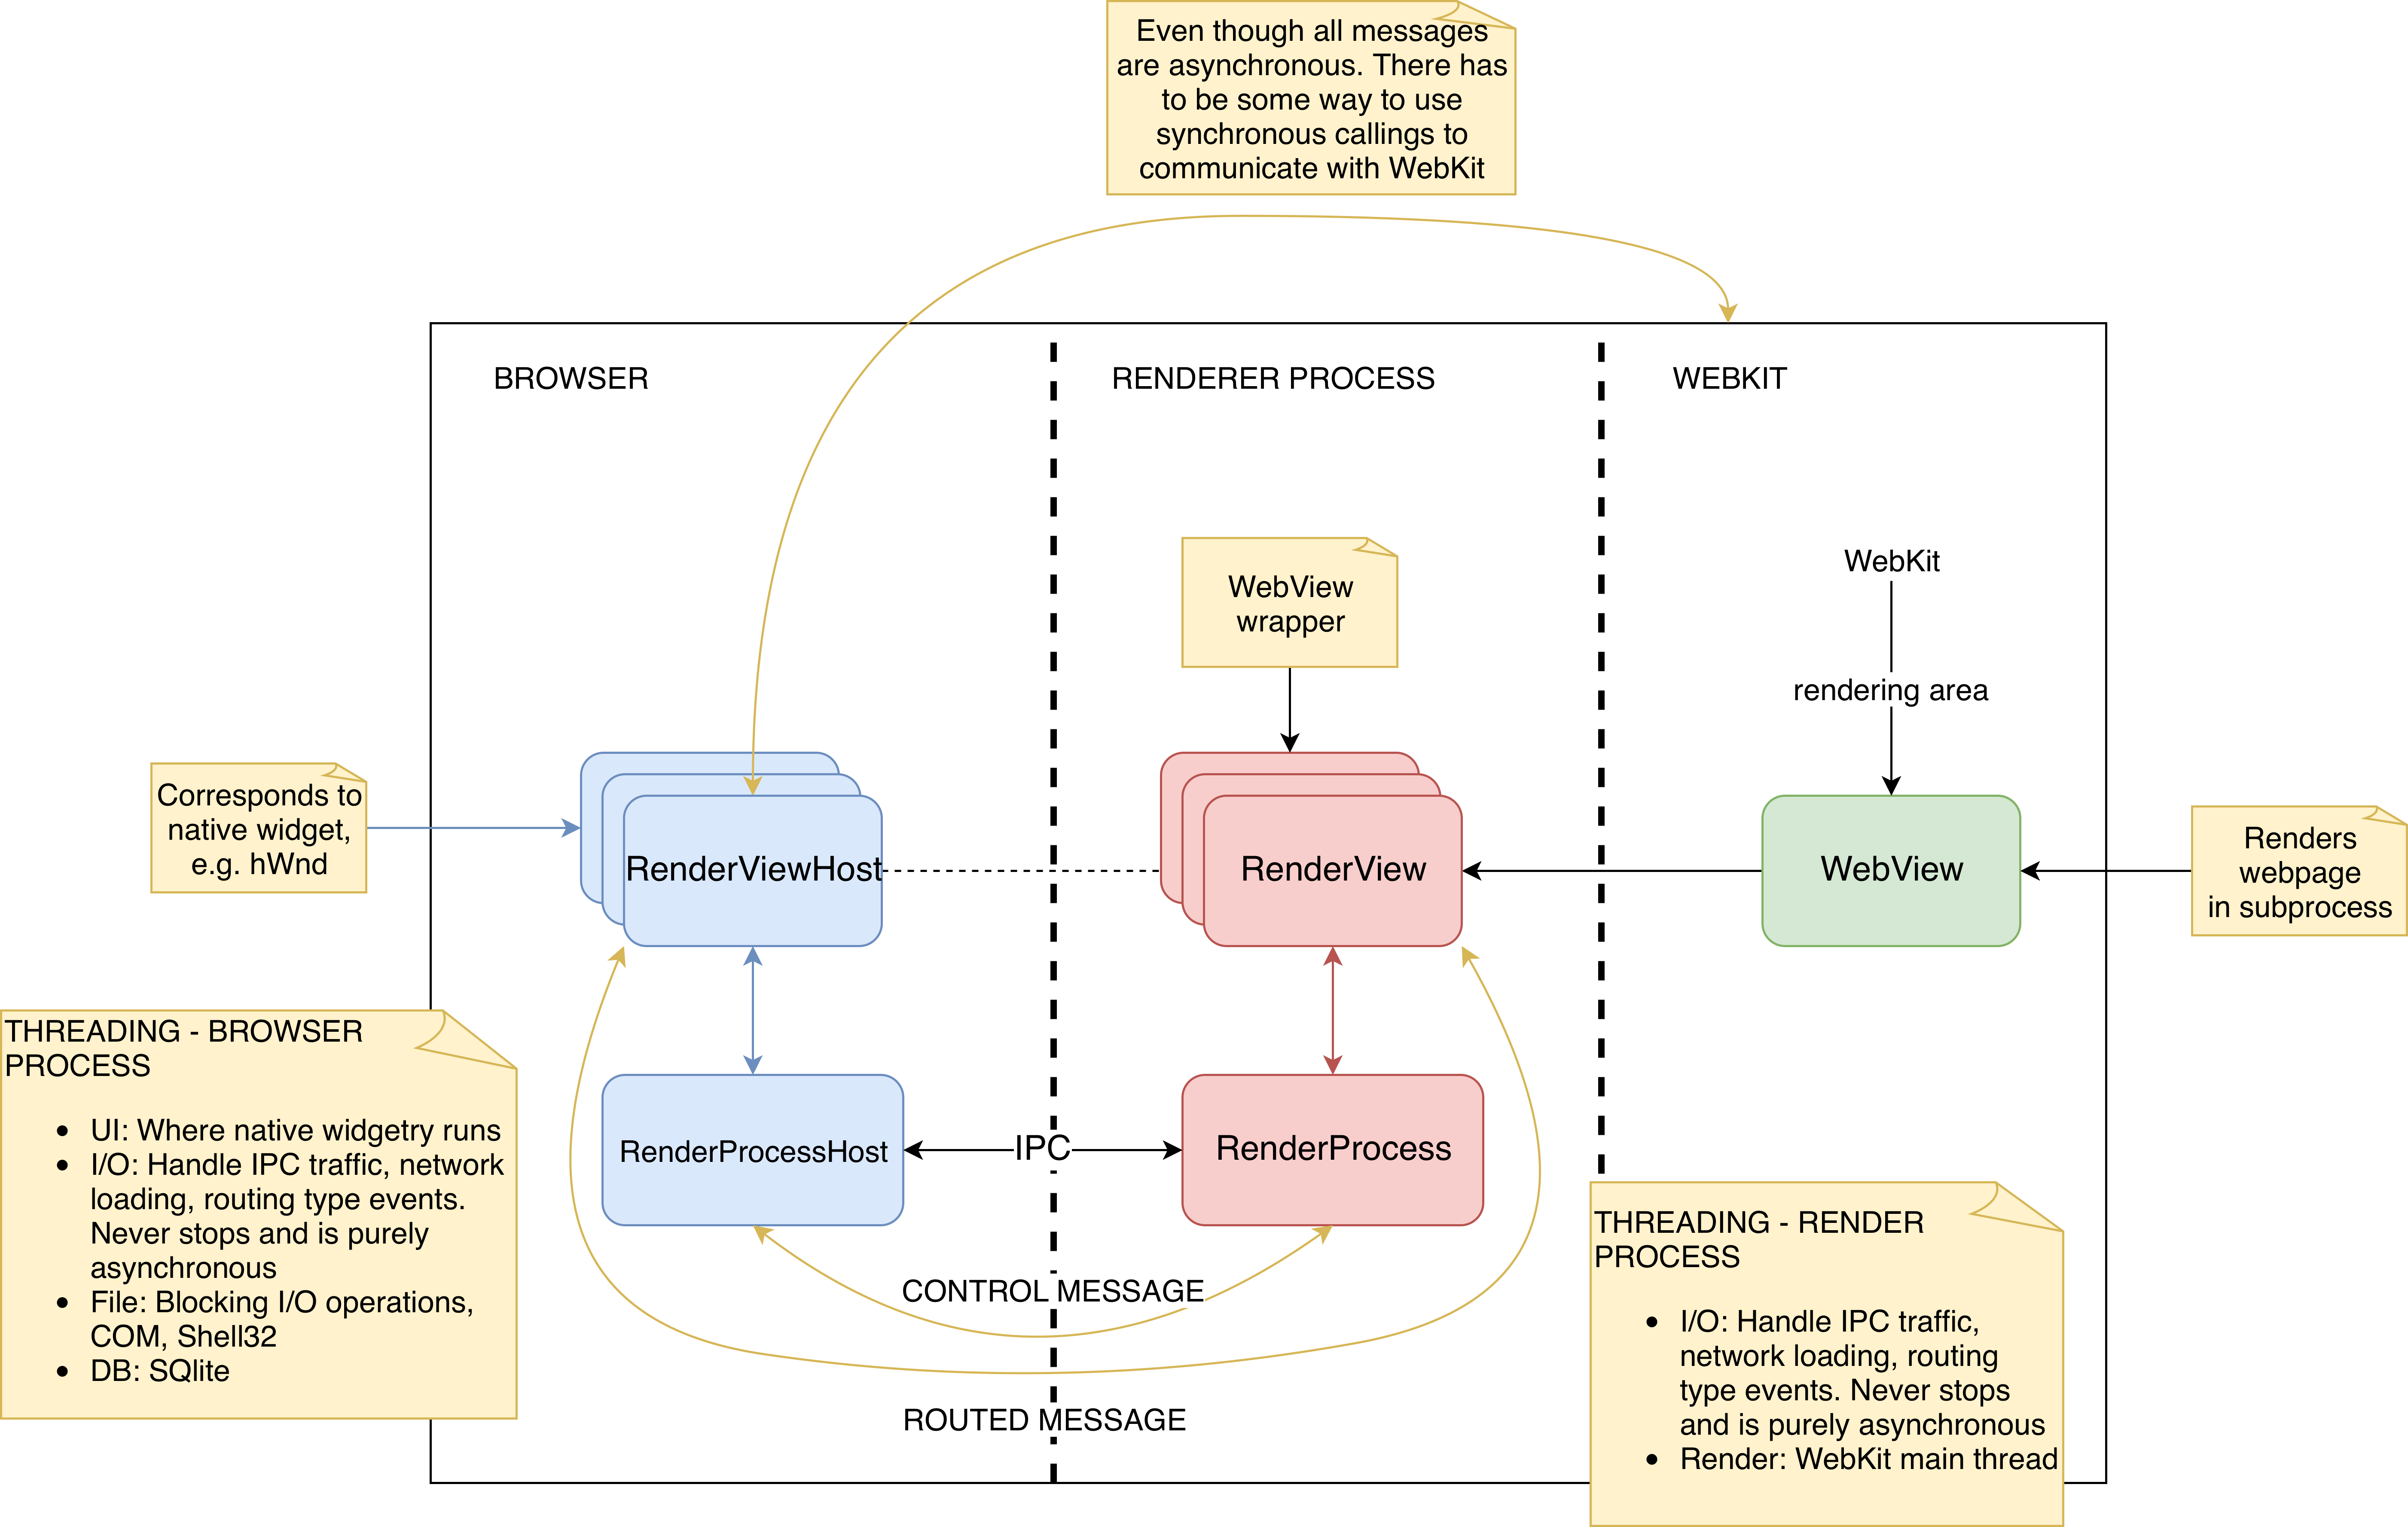
\includegraphics[width=\textwidth]{img/multiprocess.png}
    \caption{Chromium's multi process architecture}
    \label{fig:arch}
\end{sidewaysfigure}

Each render process has one or more \texttt{RenderView} objects, managed by the \texttt{RenderProcess}, which correspond to tabs of content. The corresponding \textit{RenderProcessHost} maintains a \texttt{RenderViewHost} corresponding to each view in the renderer. Each view is given a view ID that is used to differentiate multiple views in the same renderer. These IDs are unique inside one renderer but not within the browser, so identifying a view requires a \texttt{RenderProcessHost} and a view ID. Communication from the browser to a specific tab of content is done through these \texttt{RenderViewHost} objects, which know how to send messages through their \texttt{RenderProcessHost} to the \texttt{RenderProcess} and on to the \texttt{RenderView}.

\subsection{Components and interfaces}

In the render process:
\begin{description}
\item[\texttt{RenderProcess}] Handles IPC with the corresponding \texttt{RenderProcessHost} in the browser. There is exactly one \texttt{RenderProcess} object per render process. This is how all browser renderer communication happens.
\item[\texttt{RenderView}] Communicates with its corresponding \texttt{RenderViewHost} in the browser process (via the \texttt{RenderProcess}), and WebKit embedding layer. This object represents the contents of one web page in a tab or popup window.
\end{description}

\noindent In the browser process:
\begin{description}
\item[\texttt{Browser}] Represents a top-level browser window.
\item[\texttt{RenderProcessHost}] Represents the browser side of a single browser renderer IPC connection. There is one \texttt{RenderProcessHost} in the browser process for each render process.
\item[\texttt{RenderViewHost}] Encapsulates communication with the remote \texttt{RenderView}, and \texttt{RenderWidgetHost} handles the input and painting for \texttt{RenderWidget} in the browser.
\end{description}

\subsection{Process Models}

By default, the browser will spawn a new process and instruct it to create a single \texttt{RenderView}. On the other hand, the architecture also supports assigning new tabs to existing processes due to diverse reasons.

\begin{itemize}
    \item The total number of processes is too large
    \item The user already has an open process with that domain
    \item A web application opens a new window that it expects to communicate with synchronously
\end{itemize}

There are many ways that a web browser could be segmented into different OS processes, and choosing the best architecture depends on many factors, including stability, resource usage, and observations from actual usage. Chromium supports four different process models to allow experimentation, with a default model that best fits most users:

\begin{center}
    \addtolength{\leftskip} {-2cm}
    \addtolength{\rightskip}{-2cm}
    \begin{tabular}{m{0.15\textwidth}>{\centering}m{0.3\textwidth}>{\centering}m{0.3\textwidth}m{0.25\textwidth}}
    \hline
     & \textbf{Overview} & \textbf{Strengths} & \hspace*{0.8cm} \textbf{Weaknesses} \\\cline{2-4} 
    \textbf{Process$\times$site-instance} & \begin{center}One renderer process for each instance of a site\end{center} & \begin{center}$\checkmark$ Isolates content from different sites \\ $\checkmark$ Isolates independent tabs showing the same site\end{center} & \begin{center}$\times$ More memory overhead\end{center} \\ \cline{2-4} 
    \begin{center}\textbf{Process$\times$site}\end{center} & \begin{center}Groups all instances of the same site into the same process.\end{center} & \begin{center}$\checkmark$ Less memory overhead \\ $\checkmark$ Isolates content from different sites\end{center} & \begin{center}$\times$ Can result in large renderer processes\end{center} \\ \cline{2-4} 
    \begin{center}\textbf{Process$\times$tab}\end{center} & \begin{center}One renderer process to each unit of related browsing contexts tabs (e.g: a tab and any other tabs that it opens using \textit{Javascript})\end{center} & \begin{center}$\checkmark$ Simple to understand\end{center} & \begin{center}$\times$ Leads to undesirable fate sharing between pages\end{center} \\ \cline{2-4} 
    \begin{center}\textbf{Single process}\end{center} & \begin{center}For the purpose of comparison\end{center} & \begin{center}$\checkmark$ Easy to implement \\ $\checkmark$ Good for developing purposes \end{center} & \begin{center}$\times$ Not safe nor robust\\ $\times$ Any renderer crash will cause the loss of the entire browser process\end{center} \\ \hline
    \end{tabular}
\end{center}

\subsection{Threading and Inter-process Communication}

Within the browser, communication with the renderers is done in a separate I/O thread. Messages to and from the views then have to be proxied over to the main thread using a \texttt{ChannelProxy}. The advantage of this scheme is that resource requests, which are the most common and performance critical messages, can be handled entirely on the I/O thread and not block the user interface. These are done through the use of a \texttt{ChannelProxy::MessageFilter} which is inserted into the channel by the \texttt{RenderProcessHost}. This filter runs in the I/O thread, intercepts resource request messages, and forwards them directly to the resource dispatcher host. 

Each renderer also has a thread that manages communication (in this case, the main thread), with the rendering and most processing happening on another thread (see the diagram in multi-process architecture). Most messages are sent from the browser to the WebKit thread through the main renderer thread and vice-versa. This extra thread helps support synchronous renderer-to-browser messages.

\subsection{Security point of view}

Chromium's mechanism \cite{sec} for separating running renderers, mitigates system failures or vulnerabilities from spreading, thus, helping protect against malware. For example, it can ensure that the renderer's only access to the network is via its parent browser process. Likewise, it can restrict its access to the filesystem using the host operating system's built-in permissions.

In addition to restricting the renderer's access to the filesystem and network, it can also place limitations on its access to the user's display and related objects, which prevents a compromised renderer from opening new windows or capturing keystrokes. 


\section{Plugin architecture} 
\label{sec:plugin}

Plugins are a major source of browser instability. Plugins also make sandboxing impractical, as plugins are written by third-parties and we can't control their access to the operating system. The solution is to run plugins in their own separate process. Chromium has the ability to run plugins both in process, which is handy for testing, as well as out of process. 
\subsection{In process plugins}
\begin{figure}[H]
    \centering
    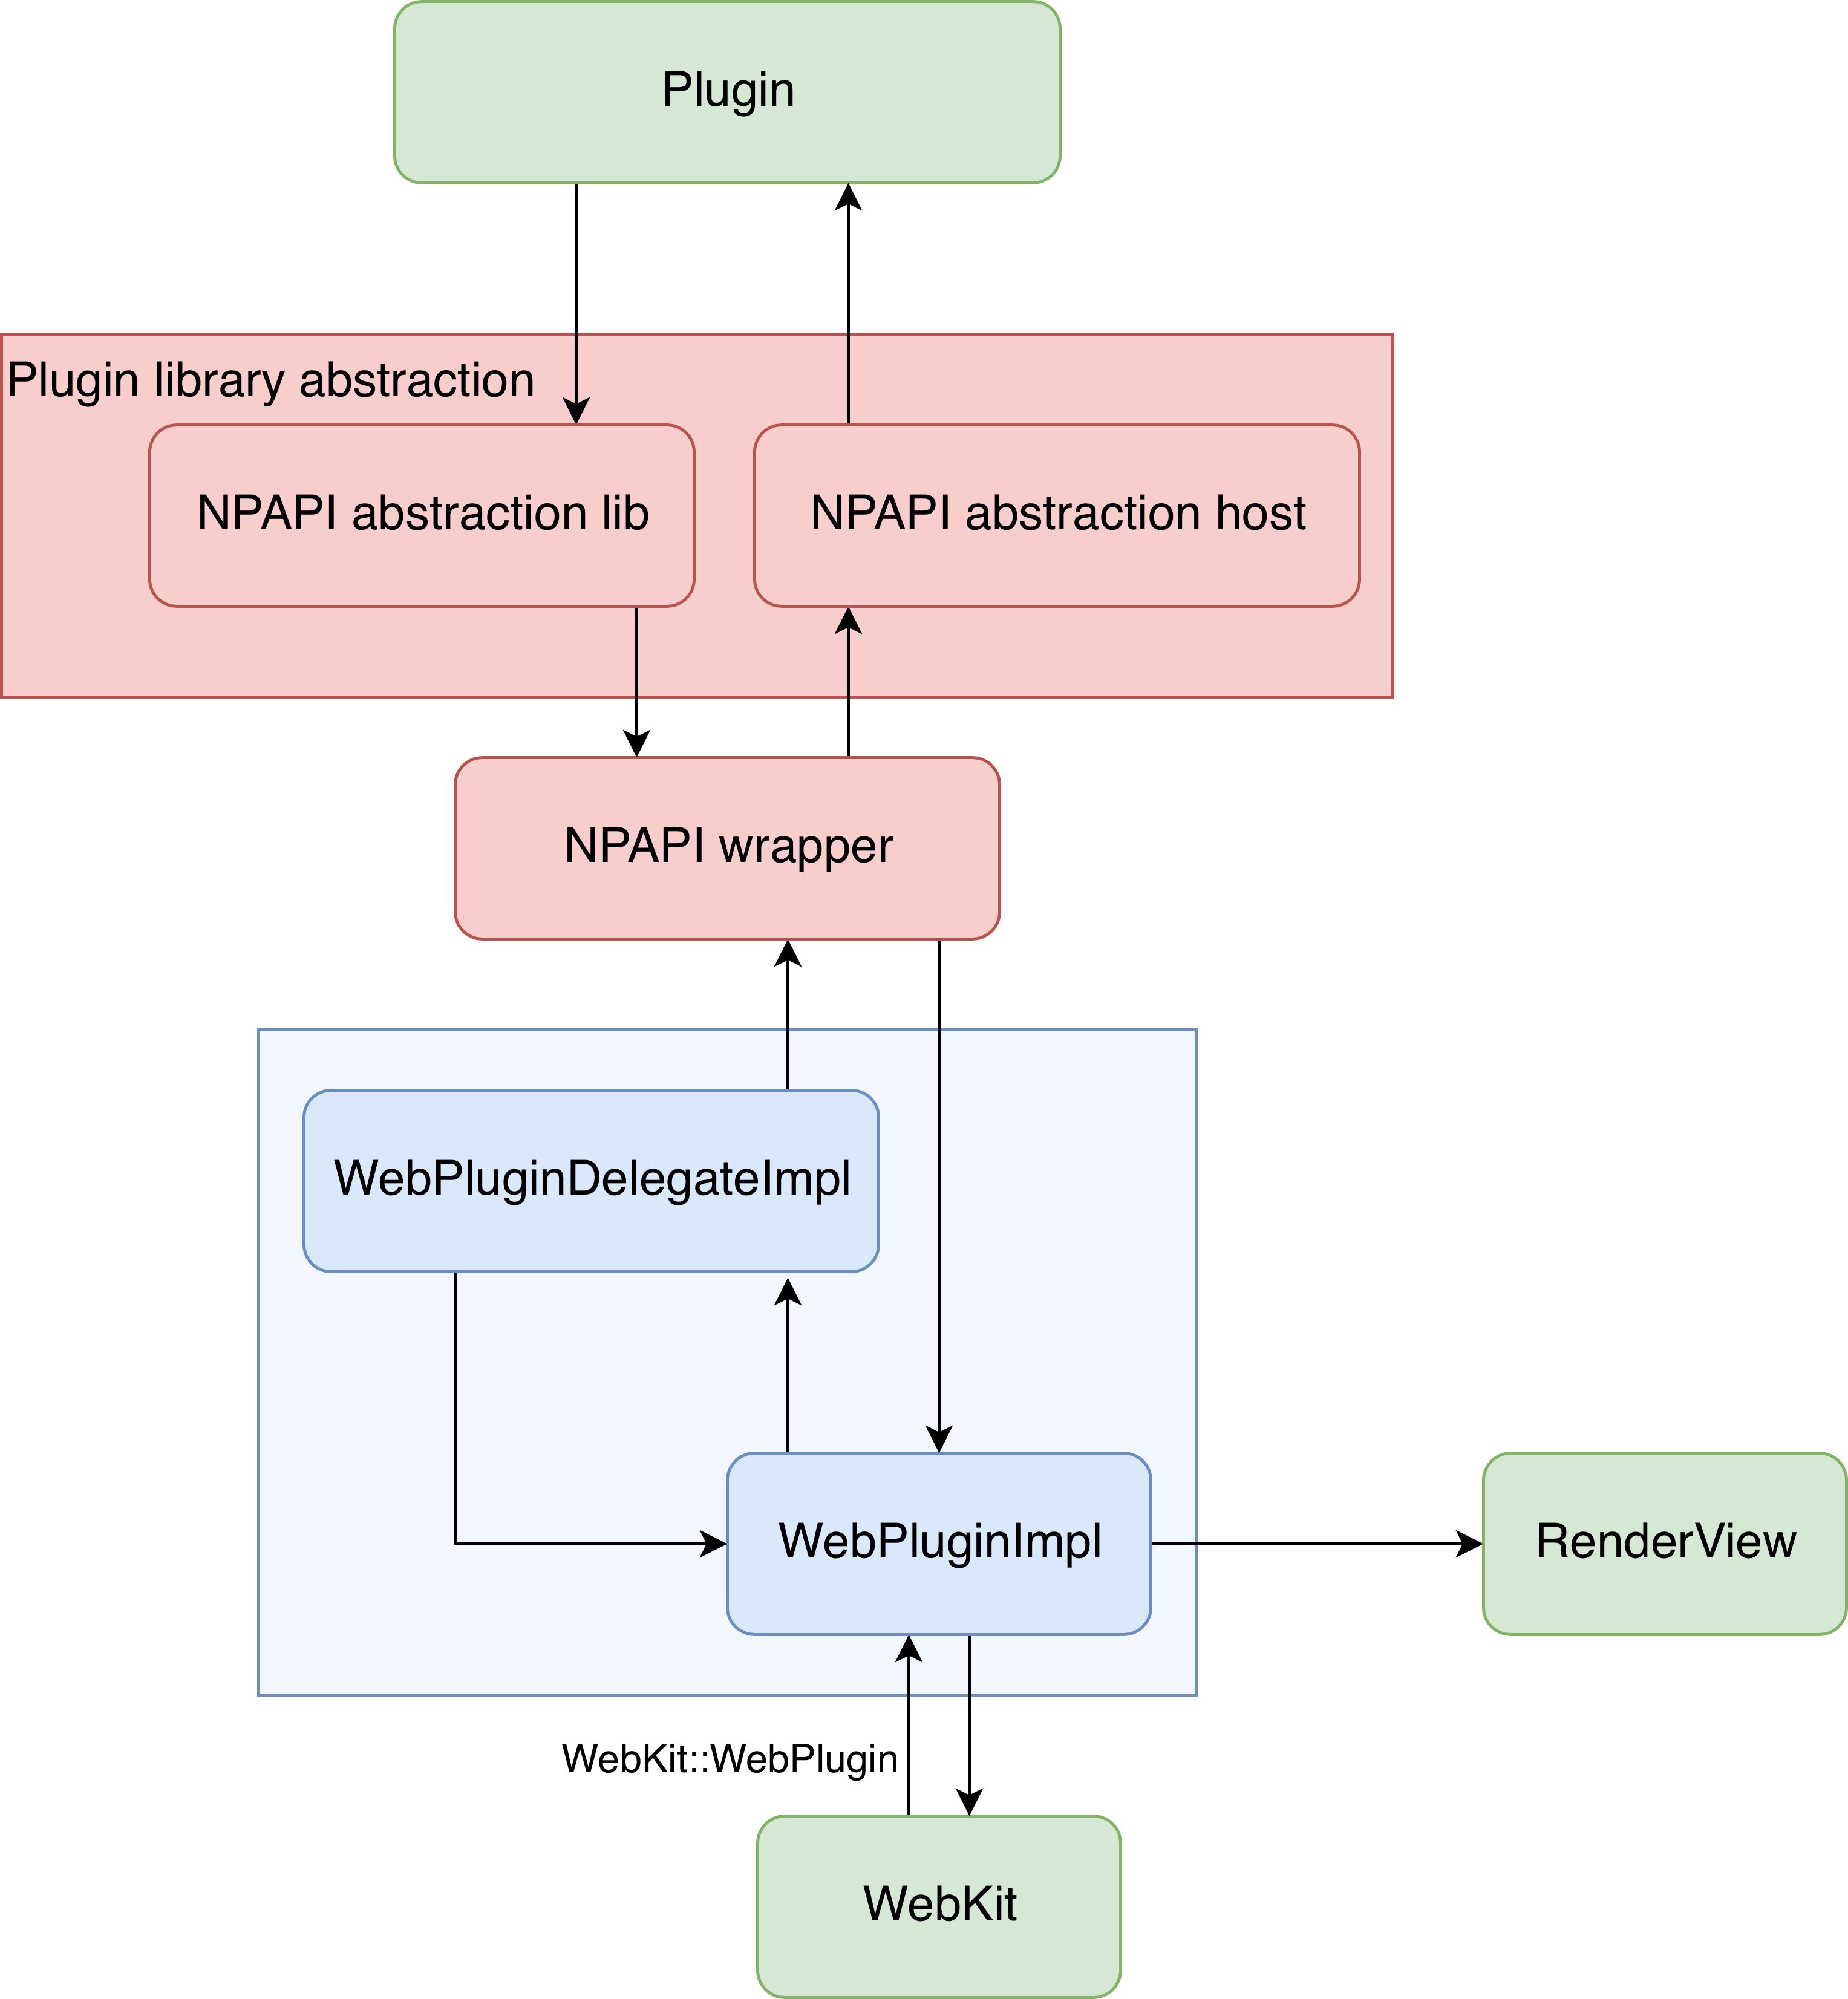
\includegraphics[width=0.8\textwidth]{img/in.png}
    \caption{In process plugin}
    \label{fig:in}
\end{figure}

WebKit embedding layer expects the embedder to implement the \texttt{WebKit::WebPlugin} interface. This is implemented by \texttt{WebPluginImpl}. The WebPluginImpl talks ``up" the chain to a \texttt{WebPluginDelegate} interface. This in turn talks to our NPAPI wrapper layer. Figure \ref{fig:in} represent the aforementioned description.

\subsection{Out of process plugins}

The layer indicated by the dotted line in figure \ref{fig:out} interposes an IPC cover between the \texttt{WebPluginImpl} and \texttt{WebPluginDelegateImpl} layers seen in figure \ref{fig:in}. The two sides of the \texttt{Renderer/Plugin} communication channel are represented by the \texttt{Channel} and the \texttt{ChannelHost} components. Since each unique plugin may be present in many renderer processes, this means there must be one \texttt{ChannelHost} for each type of plugin it uses. Similarly, every plugin process has a Channel component for each renderer process.

\begin{figure}[H]
    \centering
    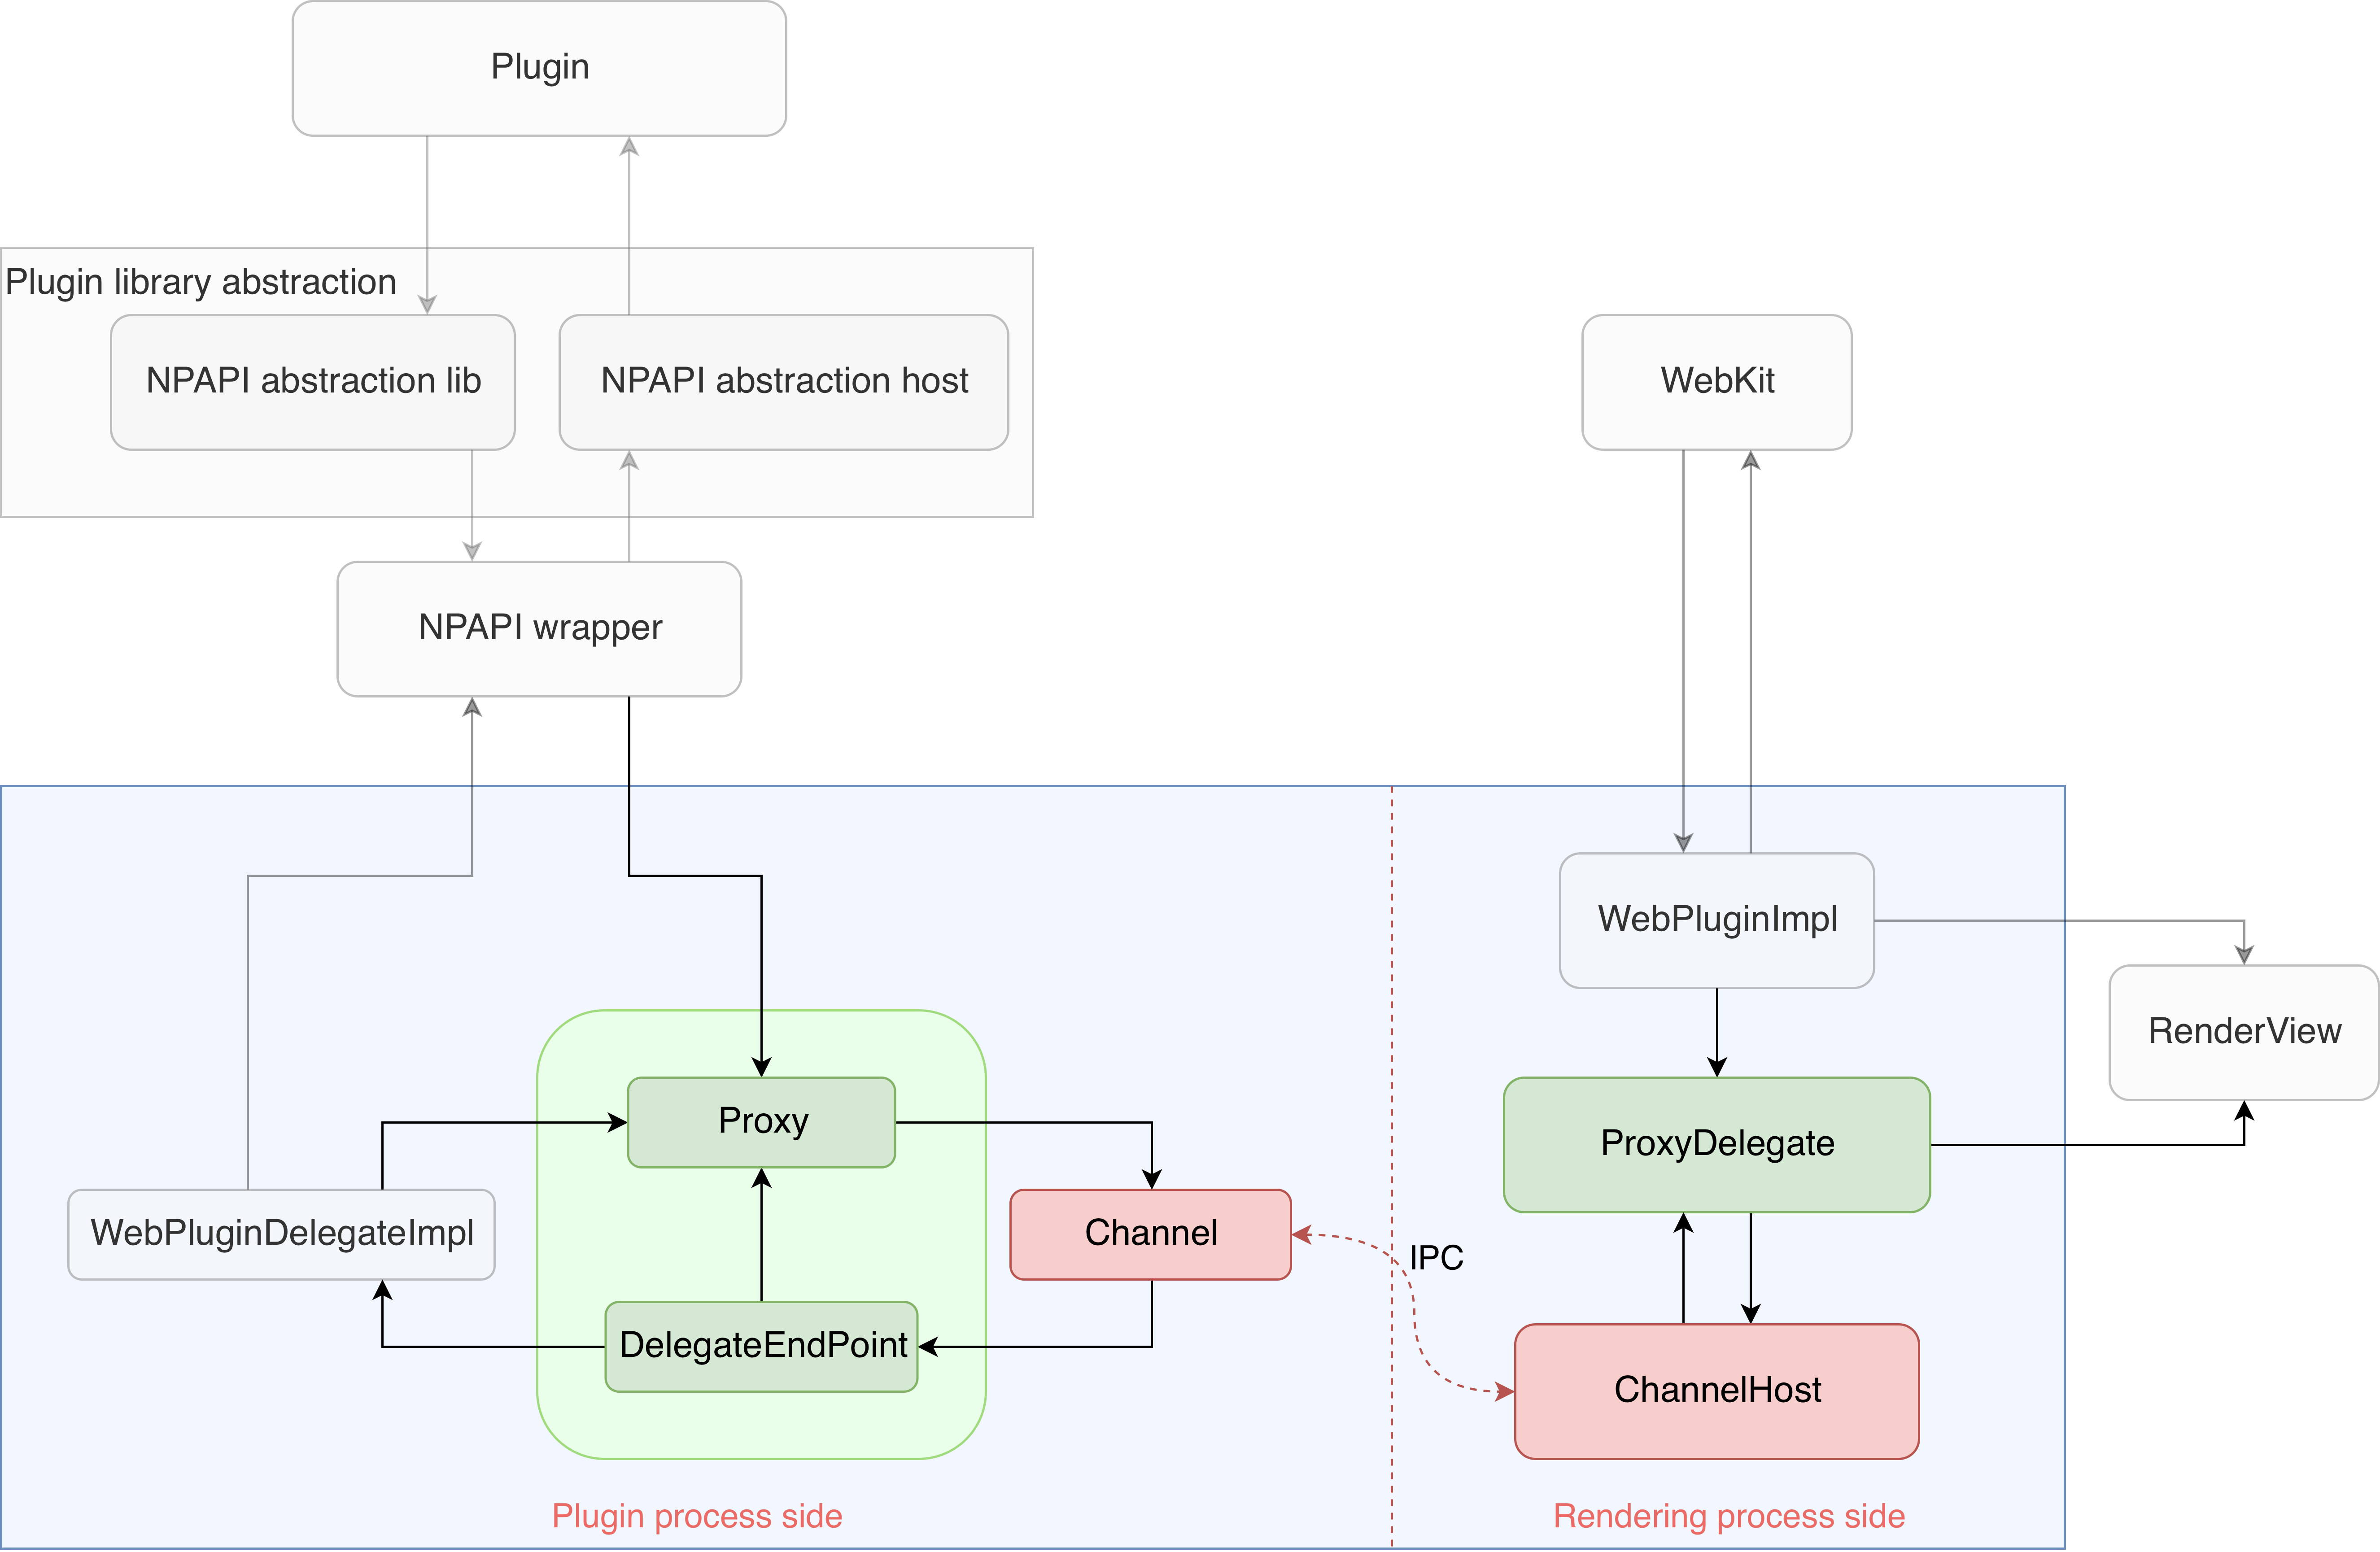
\includegraphics[width=\textwidth]{img/chromium-out.png}
    \caption{Out of process plugin}
    \label{fig:out}
\end{figure}

Each end of the channel, in turn, maps to many different instances of a plugin. The channel is in charge of multiplexing the communication between these many objects over one IPC connection.


\section{Alternative architecture}

From the standpoint of the aforementioned concepts, where we summarize the multi-process architecture's main advantages, we found that there is no other architecture that could replace this one maintaining its core functionalities, that synergize so well with the project philosophy.

Therefore, and under our humble point of view, this architecture is a perfect counterpart and the main motive as to why the application achieves its purposes and user expectatives.
\chapter{Software design}
\label{chap:design}

\myepigraph{If it were the case that putting effort into design reduced the effectiveness of programming I would be against it.}{Martin Fowler}{DesignStaminaHypothesis}


We focused on analyzing the 125 files that form the IPC tree of the Chromium GitHub repository \footnote{\url{https://github.com/chromium/chromium/tree/master/ipc}}. Chrome processes communicate with each other via an Inter-Process Communication IPC messaging framework built into the browser. For Windows, \textit{``named pipes"} are utilized, whereas linux builds use local Unix sockets. Most of the code that implements the IPC framework is located within the \texttt{ipc/} directory in the Chrome source tree.\\ 

\noindent The following sections delve into this framework's functionalities.
\begin{sidewaysfigure}
    \centering
    \hspace*{-2.5cm}
    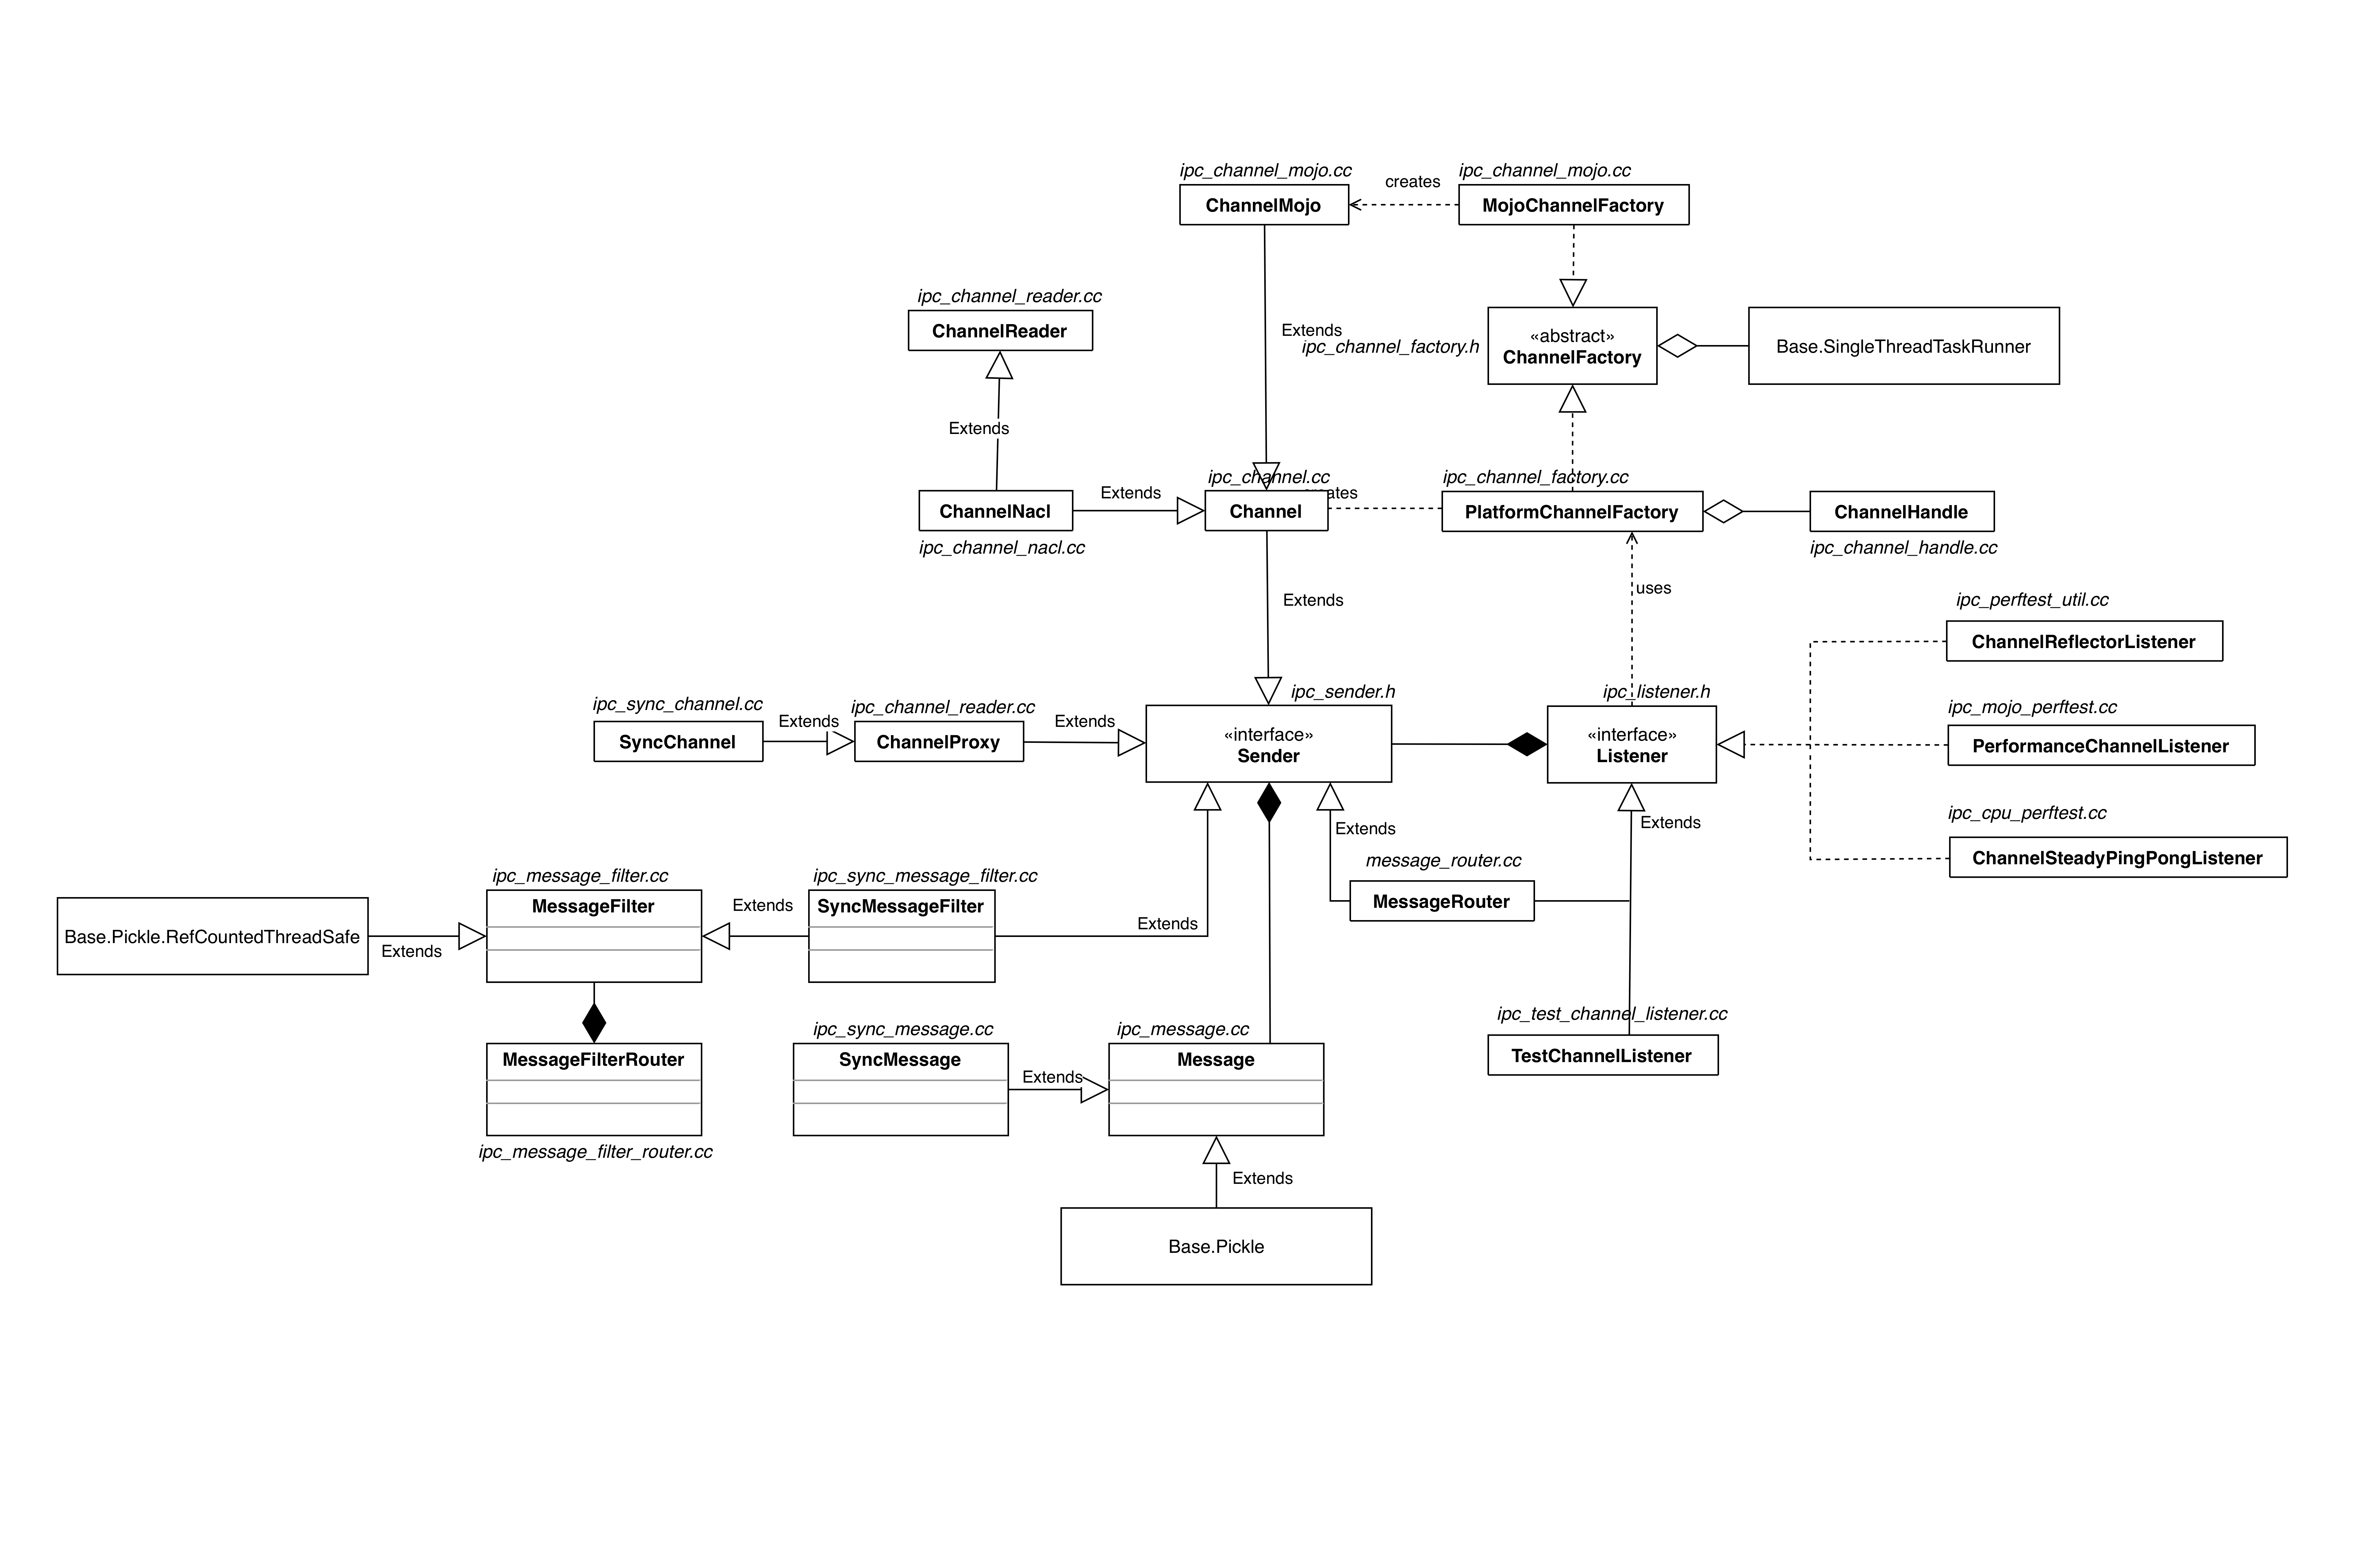
\includegraphics[width=1.2\textwidth]{img/design_min.png}
    \caption{Chromium's IPC design}
    \label{fig:design}
\end{sidewaysfigure}
\section{Channels}
The messaging framework provided by Chrome provides bidirectional communication channels between two processes through the use of a Channel object \footnote{Defined in \texttt{ipc/ipc$\_$channel.cc}}. The Channel object has one key member objects of interest to us: A listener object whose \texttt{OnMessageReceived()} function is invoked whenever a message is successfully received from the communication channel. The class definition of Listener is defined in \texttt{ipc/ipc$\_$listener.h}, but several other classes derive from it. A \texttt{Listener} object is a special object that is associated with a channel that handles incoming messages. It is used to provide the desired functionality of a given process by exposing a number of method callbacks that are invoked via the \texttt{Listener::OnMessageReceived()} function. This function typically does not handle many of the messages it receives itself; instead, it routes the messages to one of a series of objects that has been previously registered with the Listener object in question. Each of these objects registered to the listener are uniquely identified by a routing ID, and contain a series of numbered callback methods that clients may invoke. The number of the callback is unique to each object and is referred to as a message type. In the case of the browser process, the Listener object maintains a list of \texttt{MessageFilter} objects. Figure \ref{fig:design} shows the described class arrangement.


\section{Messages}

The basic unit for transmission across IPC channels is the Message object (defined in \texttt{ipc/ipc$\_$message.h}). Message objects are structured as follows:

Messages are processed in the order they are received from the communications channel by the \texttt{ChannelReader::ProcessIncomingMessage()} function \footnote{Implemented within \texttt{ipc/ipc$\_$channel$\_$reader.cc}}. Once messages have been successfully received, they are routed to an appropriate callback function through the use of a routing ID and message type, both of which are present in the Message header. The remainder of the message data is interpreted as a set of parameters for the called function, or for results of a called function in the case of reply messages.

\subsection{Types of messages}

There are two primary types of messages: ``routed" and ``control". 

\begin{description}
\item[Control] These messages are handled by the class that created the pipe. Sometimes that class will allow others to received messages by having a MessageRouter \footnote{Implemented in \texttt{ipc/message\_router.cc}} object that other listeners can register with and received ``routed" messages sent with their unique id. This is displayed in figure \ref{fig:observer}.

\item[Routed] Used to get messages to a specific RenderViewHost. 
\end{description}

\noindent Independent of the message type is whether the message is sent from:

\begin{description}
\item[Browser $\Longrightarrow$ renderer] Called Frame messages because they are being sent to the RenderFrame. 
\item[Renderer $\Longrightarrow$ browser] Called FrameHost messages because they are being sent to the RenderFrameHost.
\end{description}

\subsection{Sending messages}

Messages are sent through ``channels". In the browser, the RenderProcessHost contains the channel used to send messages from the UI thread of the browser to the renderer. Messages are sent by pointer and will be deleted by the IPC layer after they are dispatched.

\subsection{Message macros}

Special macros are used to declare messages. Messages are handled by the \texttt{IPC::Listener} interface, the most important function on which is \texttt{OnMessageReceived}. There exist a variety of macros to simplify message handling in this function.


\section{Found software Design Patterns}

In this section we'll try to extract some Design Patterns \cite{gammaetal} from the IPC Component Design Diagram in figure \ref{fig:design}.

\subsection{Adapter pattern}

The adapter design pattern is one of the twenty-three well-known GoF design patterns. It allows the interface of an existing class to be used as another interface. It is often used to make existing classes work with others without modifying their source code. 

This example (figure \ref{fig:adapter}) is is a wrapper around an OSX Mach port that can be transported across Chrome IPC channels that support attachment brokering. The send right to the Mach port will be duplicated into the destination process by the attachment broker. When used by client code in the sender process, this class is just a wrapper. The client code calls \texttt{Send(new Message(MachPortMac(mach\_port)))} and continues with its workflow. Behind the scenes, a MachPortAttachmentMac takes ownership of the Mach port. 
\begin{figure}[H]
    \centering
    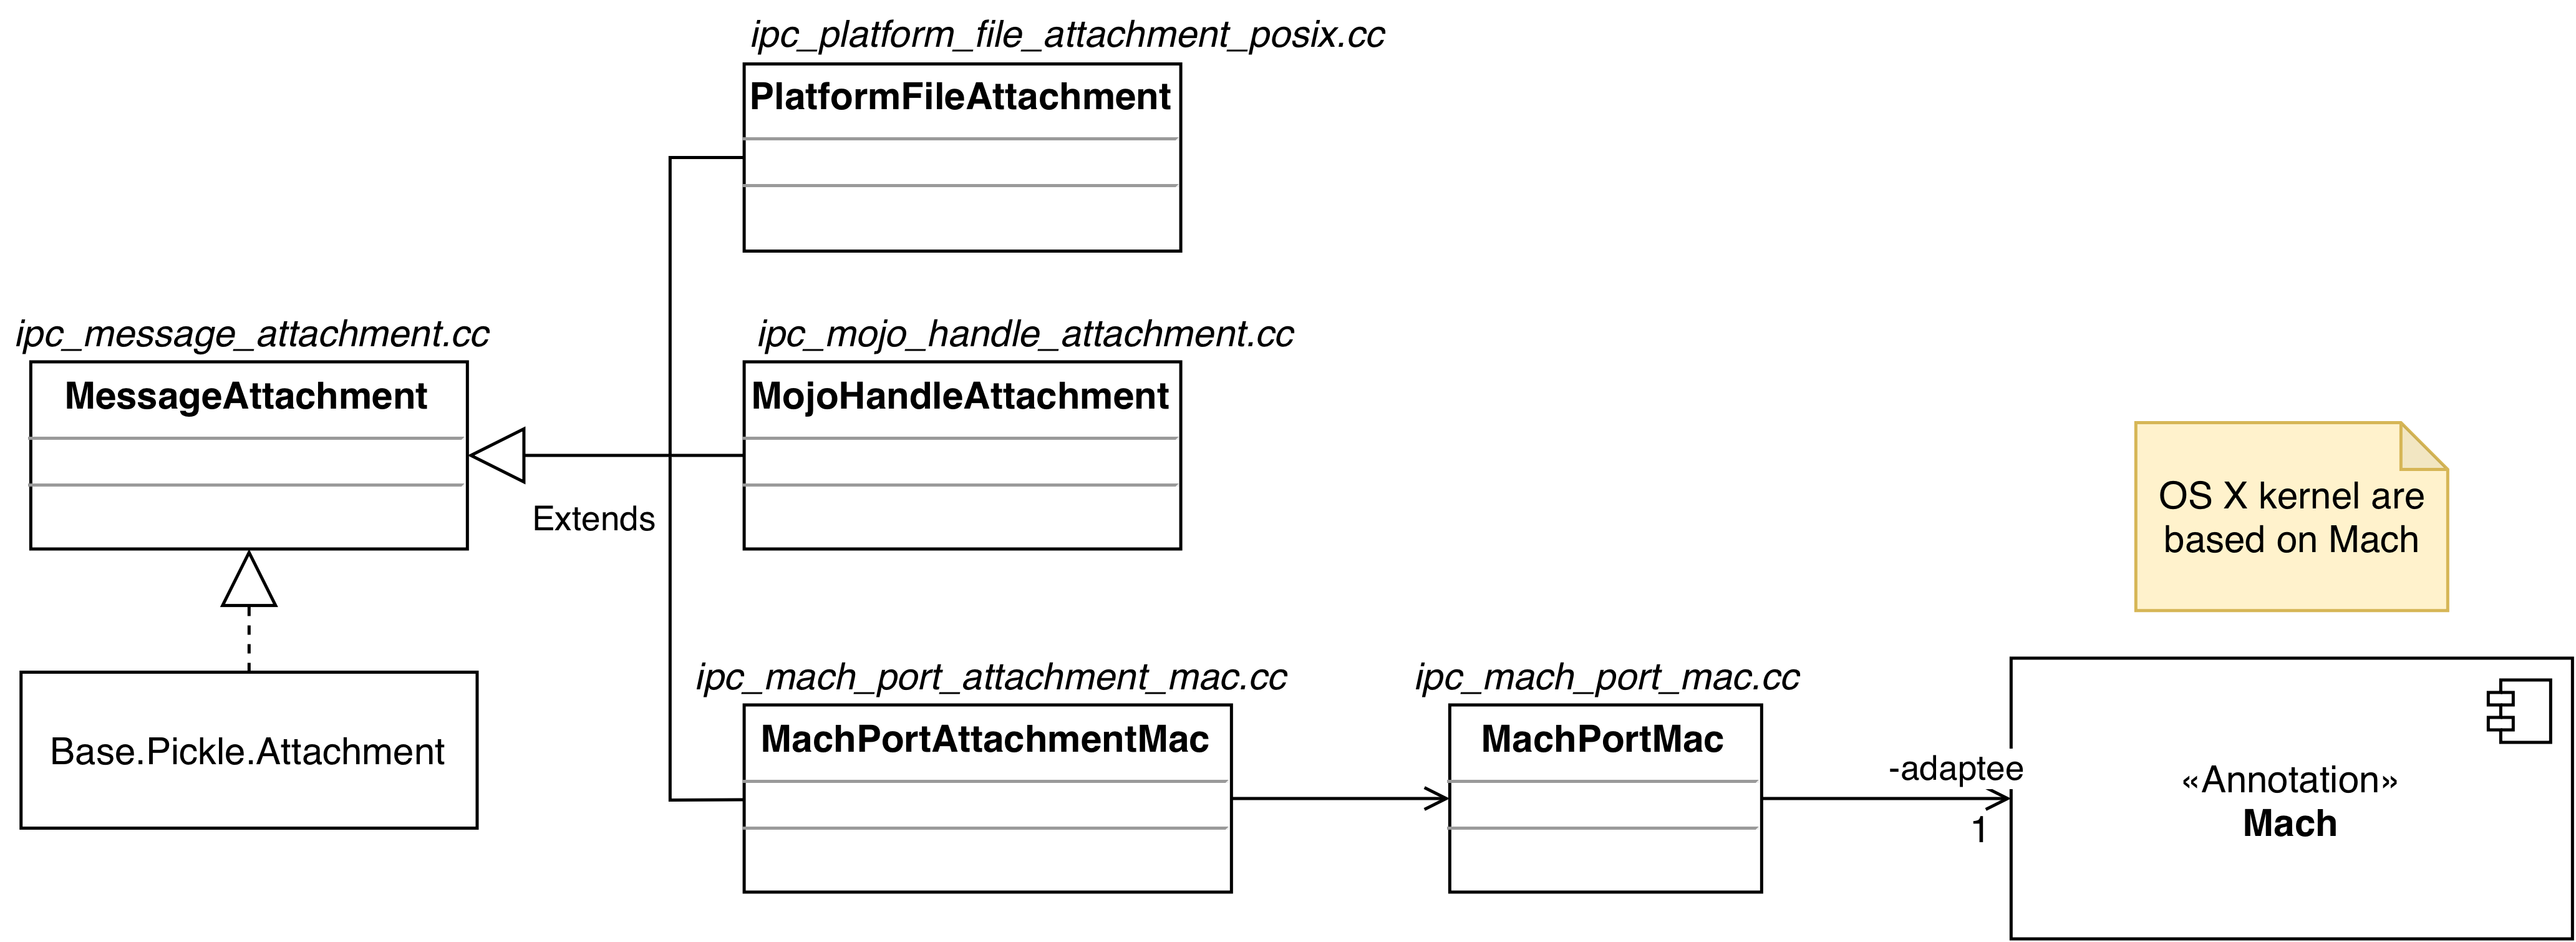
\includegraphics[width=\textwidth]{img/adapter.png}
    \caption{Adapter Pattern used to wrap OSX Mach}
    \label{fig:adapter}
\end{figure}

\subsection{Observer pattern}

\begin{sidewaysfigure}
    \centering
    {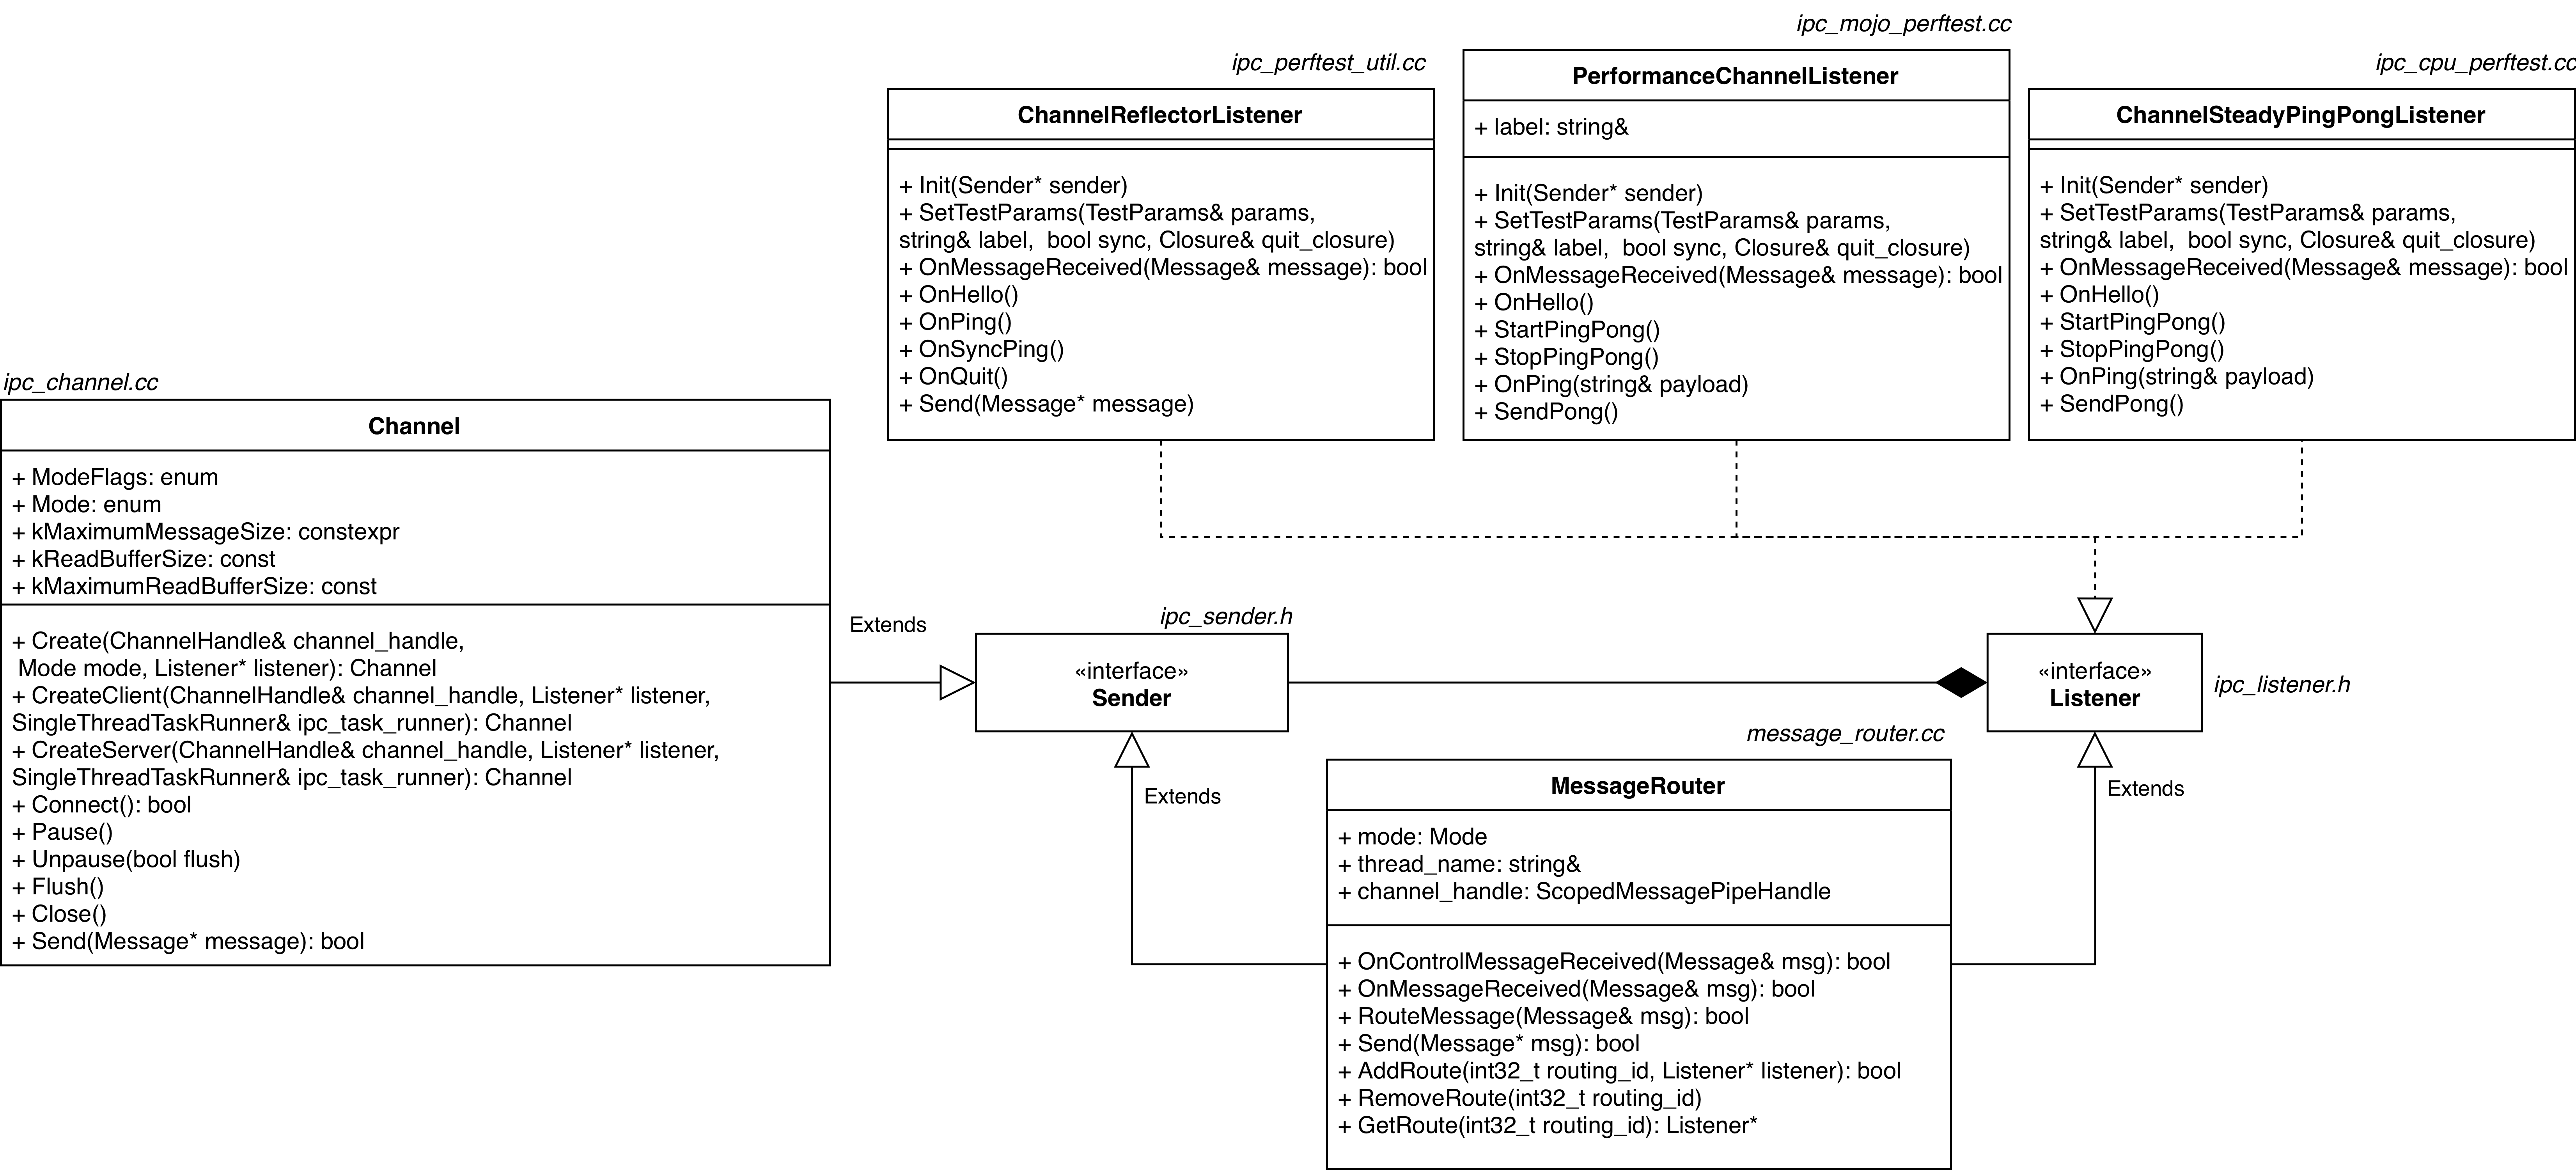
\includegraphics[width=\textwidth]{img/observer.png}}
    \caption{Observer Pattern used so listeners can register and receive messages}
    \label{fig:observer}
\end{sidewaysfigure}


In this example (figure \ref{fig:observer}), observer pattern is mainly used to implement an event handling system, where two main actor classes can be clearly identified:
\begin{description}
    \item[Subject] This component has methods to register and detach listeners to events.
    \item[Observer] Dependents. List of components to be notified upon events.
\end{description}
\begin{center}
    \begin{tabular}{p{0.5\textwidth}p{0.5\textwidth}}
    \hline
    \textbf{Problem} & \textbf{Solution} \\ \hline
    One-to-many dependency can lead to tight object coupling & Subject and Observer are loosely coupled\\ \hline
    Upon one object state change a unknown number of dependent objects must be updated & Using Subject and Observer ensures all registered observers are notified and updated\\ \hline
    one object can notify an open-ended number of other & Subject responsibility is to maintain a list of observers\\ \hline
    \end{tabular}
\end{center}

\subsection{Factory pattern}

\begin{figure}[H]
    \centering
    \makebox[\textwidth][c]{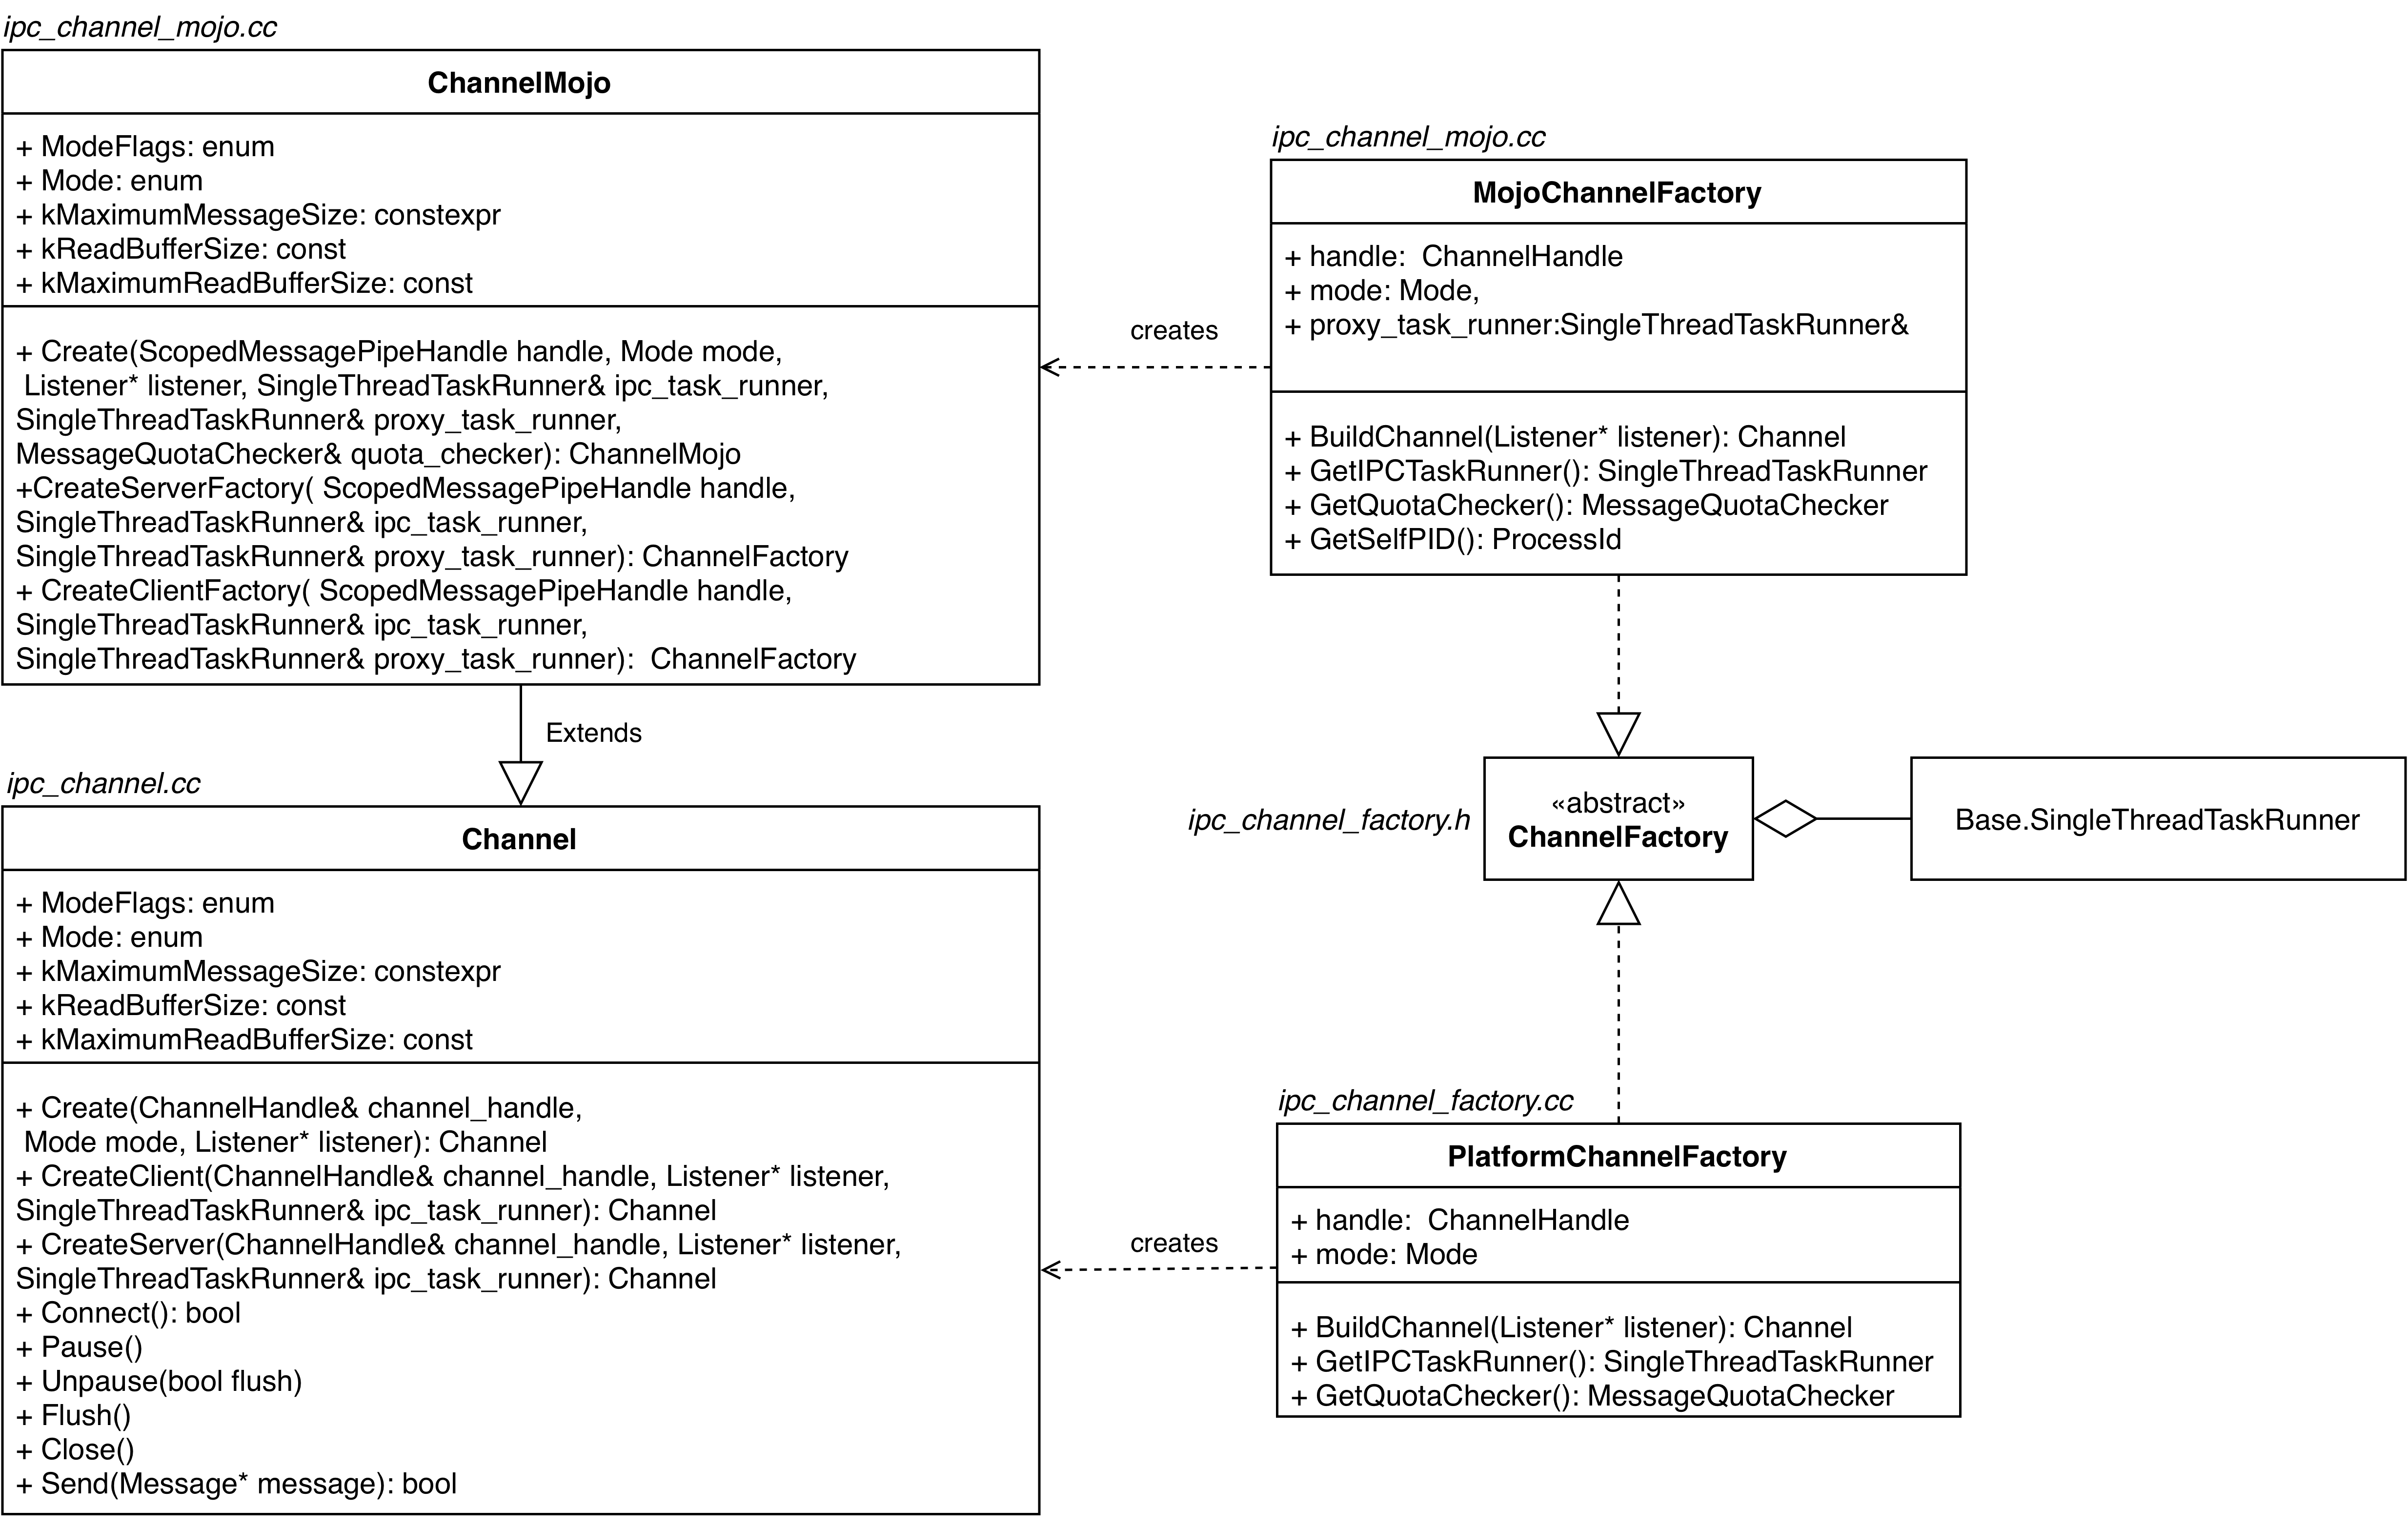
\includegraphics[width=1.2\textwidth]{img/factory.png}}
    \caption{Factory Pattern used to instantiate different channels}
    \label{fig:factory}
\end{figure}


\section{Design alternatives} 
\label{sec:bridge}

We propose the possibility using a bridge pattern to decouple several abstractions from their platform dependant implementations. 

One example can be seen in figure \ref{fig:alt}, where we found that \texttt{MojoChannelFactory's getPid} implementation depends on the platform and is currently using \texttt{ifdef} logic chains for its implementation.
\begin{sidewaysfigure}
    \centering
    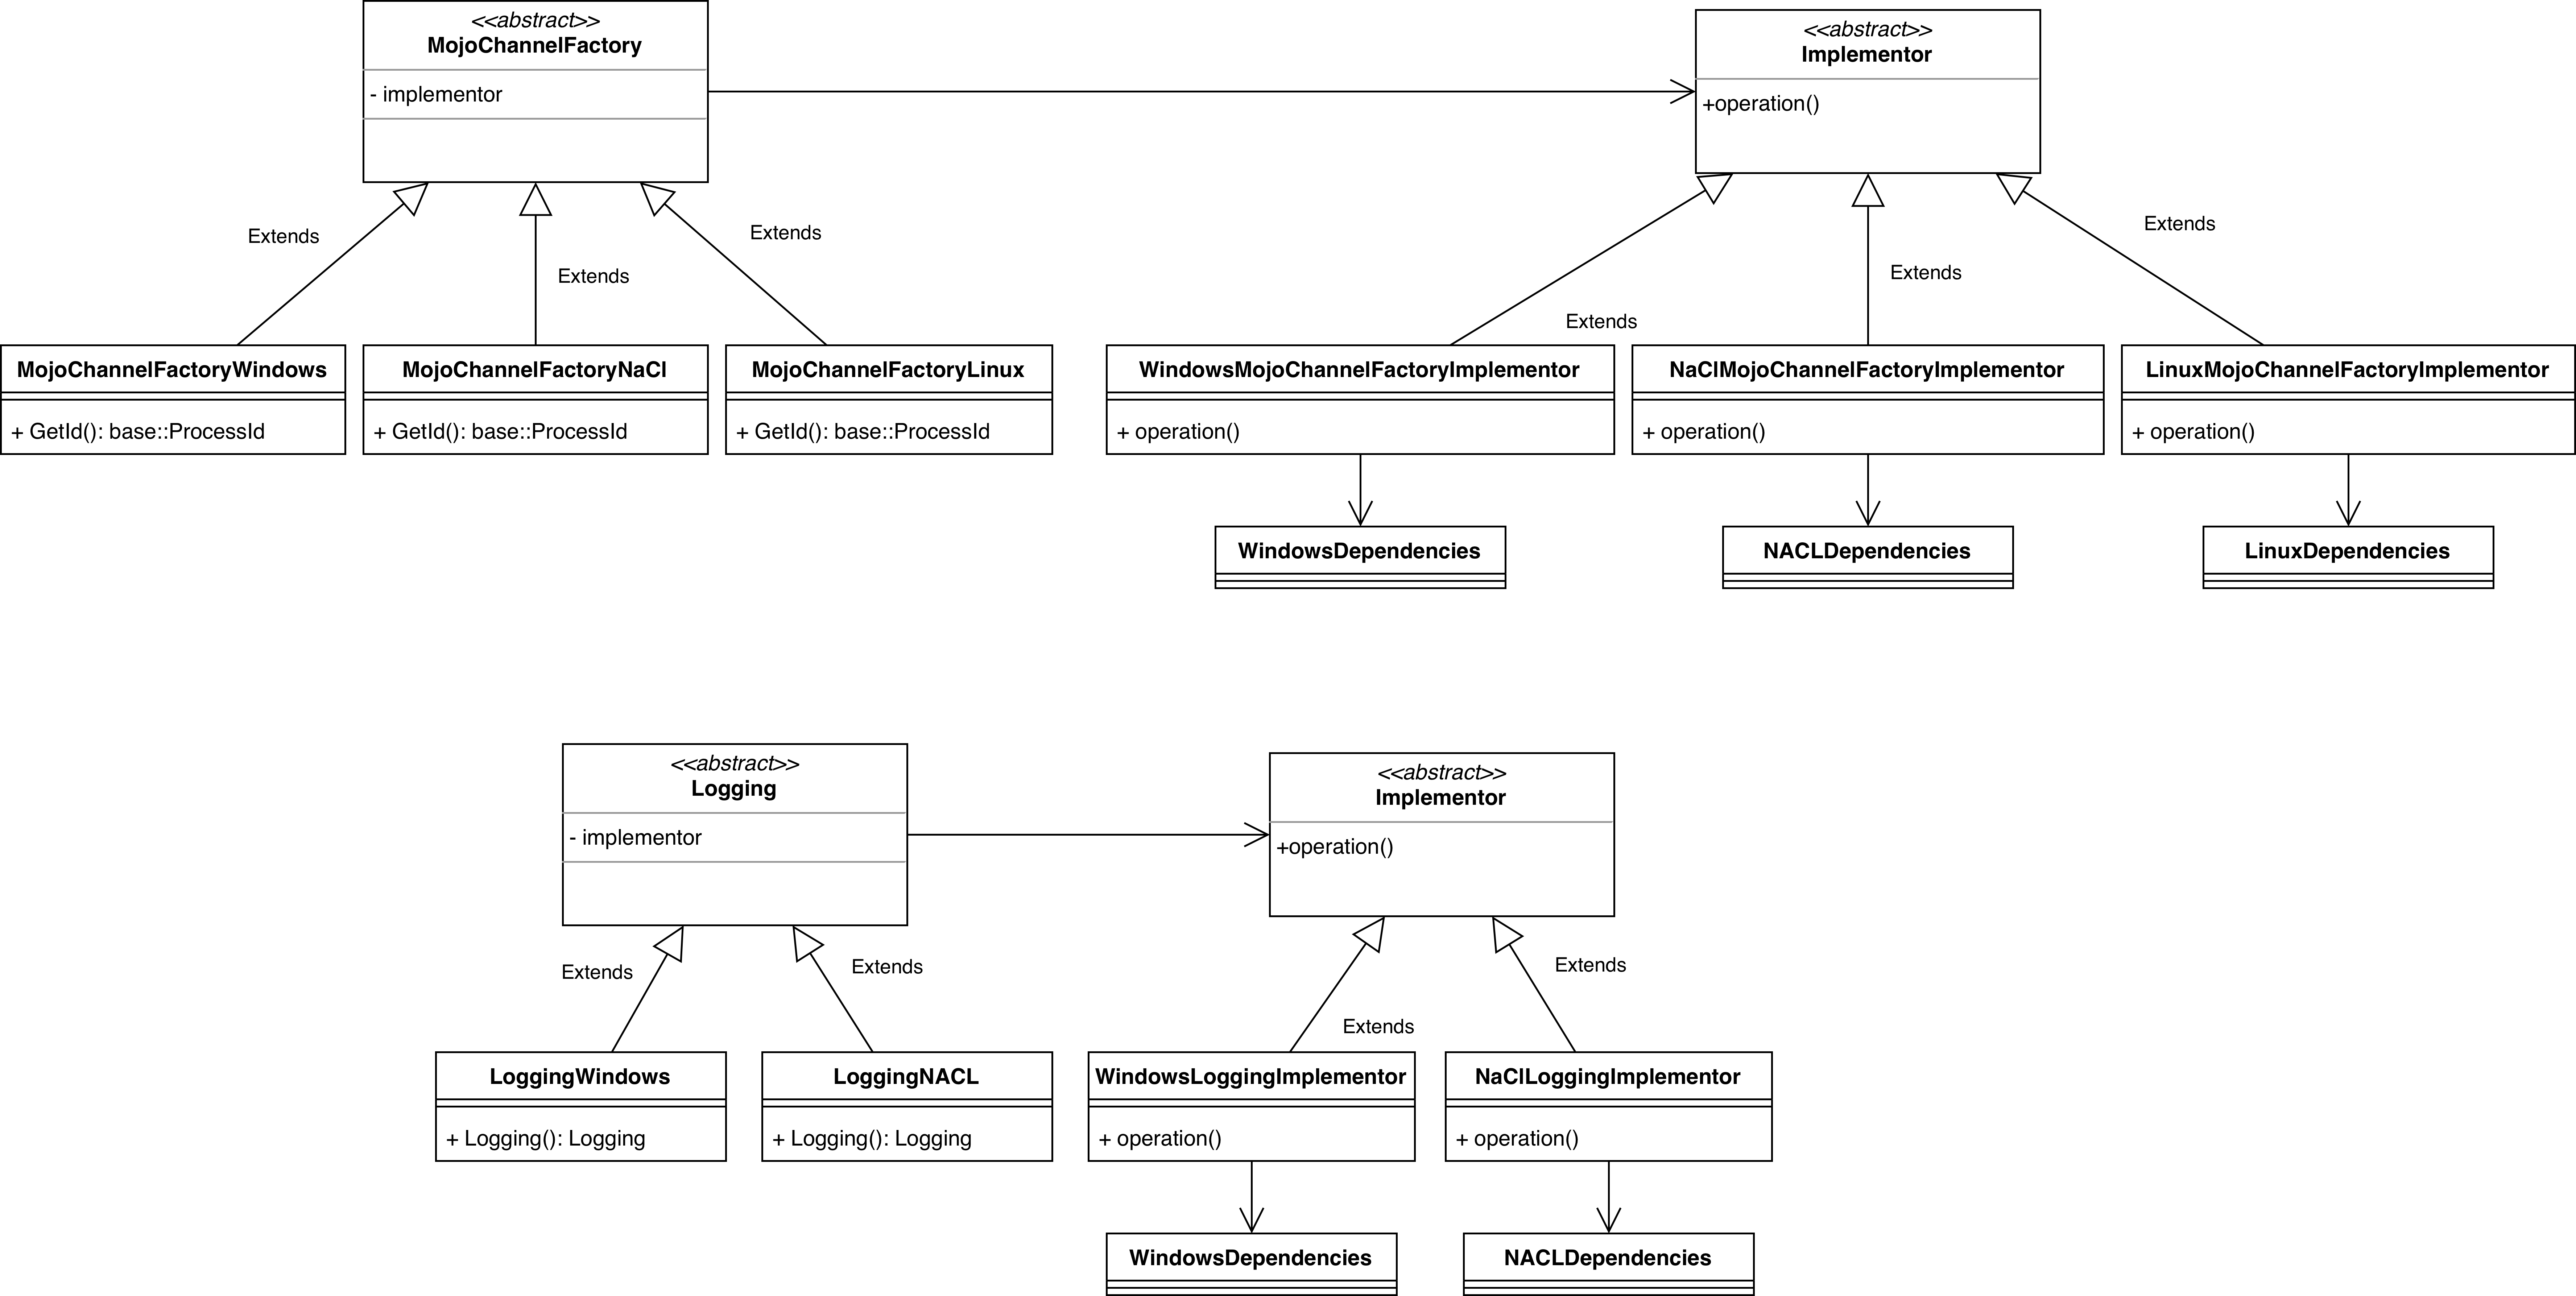
\includegraphics[width=\textwidth]{img/alt.png}
    \caption{Alternative design to decouple Logging and MojoChannelFactory abstraction from their different platform implementations}
    \label{fig:alt}
\end{sidewaysfigure}
\chapter{Software Quality}
\label{chap:quality}

\section{Metrics}

\subsection{Cohesion, coupling and connascence}

The three concepts are very related and can hint at ways to improve the quality of the software. Coupling measures how closely connected two routines or modules are. On the other hand, cohesion refers to the degree to which the elements inside a module belong together. Low coupling often correlates with high cohesion, and vice versa. Low coupling is often a sign of a well-structured computer system and a good design, and when combined with high cohesion, supports the general goals of high readability and maintainability. For this matter we are focusing in Chromium's IPC as we did in the prior section. From this standpoint we found several design patterns that help maintain loosely coupled components as well as highly coherent units.

Connascence allows reasoning about the complexity caused by dependency relationships. Two components are connascent if a change in one would require the other to be modified in order to maintain the overall correctness of the system. In parallel with the aforementioned, design patterns and the underlying idea of SOLID principles applied within the project's development assure minimum levels of connascence between components.

\subsection{Success metrics}

Any contributor should list what metrics will be used to measure the success of the new feature or change. This could be a mix of existing and new metrics. If they are new metrics, an explanation of how they will work must also be attached. If the new feature or change aims to improve performance, its impact must be measured on one of the speed launch metrics:
\begin{itemize}
    \item Loading
        \begin{itemize}
            \item Time To First Paint (FP)
            \item Time To First Contentful Paint (FCP)
            \item First Input Delay (FID) / Time to Interactive (TTI)
        \end{itemize}
    \item Animations
        \begin{itemize}
            \item Touch Scroll Start Latency (SSL)
            \item Touch Scroll Update Latency (SUL)
            \item Frame Throughput
        \end{itemize}
    \item Responsiveness
        \begin{itemize}
            \item PageLoad.InteractiveTiming.InputDelay3
        \end{itemize}
    \item Power
        \begin{itemize}
            \item Thread Times
        \end{itemize}
    \item Memory
        \begin{itemize}
            \item Browser and Renderer Memory Use
            \item OOMs
        \end{itemize}
    \item Browser UI
        \begin{itemize}
            \item Session Restore
            \item Startup
            \item Omnibox Latency
            \item Responsiveness
            \item Tab Switching
        \end{itemize}
    \item Data Use
        \begin{itemize}
            \item Traffic Size
        \end{itemize}
    \item Binary Size
\end{itemize}


\section{Documentation}

Since this is an open source project supported by thousands of contributors, the documentation is an essential part in the software development process. In this case, Chromium has an incredible amount of documentation that covers different areas such as development guides, good practices, design documents or testing and infrastructure documents.

The documentation of the project is written above Markdown files, which ones have to follow Google's style guide. When this documents are commited and reviewed, the gitiles tool is used to render HTML files from this Markdown documents. This pipeline automates the process of maintaining a web-style documentation.

The style of the design documentation is not oriented to maintain a bunch of UML diagrams (which would be very difficult given the high activity presented by the project) but to manage a textual document (which often includes some diagrams but not UML) with the following structure:
\begin{itemize}
    \item One page overview
        \begin{itemize}
            \item Summary
            \item Platforms
            \item Team
            \item Bug
            \item Code affected
        \end{itemize}
    \item Design
    \item Metrics
        \begin{itemize}
            \item Success metrics
            \item Regression metrics
            \item Experiments
        \end{itemize}
    \item Rollout plan
    \item Core principle considerations
        \begin{itemize}
            \item Speed
            \item Security
        \end{itemize}
    \item Privacy considerations
    \item Testing plan
    \item Followup work
\end{itemize}


\section{Testing}

Chromium development is heavily test driven. In order to maintain a rapid rate of development across multiple platforms and an ever increasing set of features, it is imperative that test suites be updated, maintained, executed, and evolved. Contributors are expected to write quality tests that provide ample code coverage. The Chromium Continuous Integration system is employed to run these tests 24x7. 

\subsection{Web testing}

In general, web tests involve loading pages in a test renderer and comparing the rendered output or JavaScript output against an expected output file. Blink has a large suite of tests that typically verify a page is laid out properly.  Chromium developers use them to verify much of the code that runs within a Chromium renderer.

\subsection{Unit and browser tests}

Most top-level directories of src/ have a unit test build target. Unit tests verify some part of the chromium code base in an isolated test environment, and are usually found in files with a \_unittest.cc suffix. 

Browser tests are the framework used for integration tests of Chromium. As the name implies, they run inside the browser process. The test code runs after browser process initialization and after a window has been created. Each test runs in a new browser process, to avoid tests impacting each other.
Browser tests run a full browser, and then execute a test inside the browser instance, and are usually found in files with a \_browsertest.cc suffix. 

\subsection{GPU testing}

GPU bots run a different set of tests than the majority of the Chromium test machines. Their main goal, is to specifically focus on tests which verify the correctness of Chrome's graphically accelerated rendering pipeline.

Most of the tests on the GPU bots are run via the Telemetry framework. Telemetry was originally conceived as a performance testing framework, but has proven valuable for correctness testing as well. Telemetry directs the browser to perform various operations, like page navigation and test execution, from external scripts written in Python. 

\subsection{Non-functional testing}

\subsubsection{Benchmarking}
Inside the Chromium's project, there is a group of developers known as Speed Metrics Team formed by area domain experts, focused metrics teams, devtools folks and ocassionally other experts. Whose mission is, as exposed in \cite{bench}:

\textit{``Quantify users' experience of the web to provide Chrome engineers and web developers the metrics, insights, and incentives they need to improve it."}

Their main tasks can be grouped in the following:
\begin{itemize}
    \item Quantify web UX via a high quality set of UX metrics which Chrome devs align on.
    \item Expose these metrics consistently to Chrome and Web devs, in the lab and the wild.
    \item Analyze these metrics, producing actionable reports driving our UX efforts.
\end{itemize}
This group is also responsible for ensuring that the core metrics are easy to expose and are exposed effectively. They also perform detailed analysis on key metrics and breakdown metrics, providing actionable reports on how Chrome performs in the lab and in the wild. These reports can then be used to guide regular decision making processes.

\subsubsection{Reliability tests}
The reliability bots have been providing no real results for long periods of time and are classified as deprecated as of 2019. 

The Chromium Buildbot runs a large scale set of tests called the distributed reliability tests. The reliability tests use a set of criteria to determine whether or not the build should fail. When a new crash occurs during a test, its crash dump is analyzed and a stack trace is produced for the functions that were on the stack at the point of the crash.  This stack trace is compared against a list of known crashes.  If none of the crashes in the known crashes list match the crash, the crash is considered new and the build will fail. Crash stacks for the same crash may change or have minor variants, causing them not to match any known crash and be incorrectly reported as new.  In other words, false positives are possible. 


\section{Four S}

In conclusion, the four major axis of non functional quality in Chromium are known as the four S:
\begin{description}
\item[Speed] Close attention to automated tests for speed of: rich web, page display and user interactions. 
\item[Security] Protections for users at multiple levels: sandboxed code, Safe Browsing, understandable context as well as automatical updates.
\item[Stability] Separate individual tabs and plugins into their own processes, using as many automated tests as possible.
\item[Simplicity] Simple user experience. Content, not Chromium.
    \begin{itemize}
        \item Optimal user interactions.
        \item Up-to-date software.
        \item Minimal user interruption.
    \end{itemize}
\end{description}


\section{Proposed alternatives}

\subsection{Alternative metrics}

\subsubsection{User satisfaction}
A widely used and respected metric is user satisfaction. It is a measure of how a service supplied meets or surpasses user expectation. User satisfaction is defined as the number of customers, or percentage of total customers, whose reported experience exceeds specified satisfaction goals.

\subsubsection{Halstead complexity}
This metric measures how independent the implementation of different algorithms are from their execution on a specific platform.

\subsection{Alternative documentation methods}

We believe that the current documentation model is really efficient given the size of the project. We do not see viable documentation based on diagrams and models since they would be really difficult to maintain. However, we believe in the possibility of providing diagrams and models for documentation related to higher level aspects such as architecture.

\subsection{Alternative testing}

\subsubsection{Property based testing}
Without going into too much detail, we have seen that it may make sense to use Property Based Testing tools such as RapidCheck \cite{rapidcheck}, for automatic and pseudo-random generation of test values. In addition, we assume the possibility of creating test models based on Finite State Machines that allow validating execution flows of application components, evaluating a series of post-conditions to be fulfilled when an action is executed.

\subsubsection{Formal Verification}
Since we did not deepen into concrete algorithms for complex computation issues (instead we looked upon high abstractions) we can not define or propose a formal property upon which build a proper formal verification.

\chapter{Status of the accessibility in the project}
\label{chap:accessibility}

Accessibility \cite{accessibility} often involves some design principles like using appropriate font sizes and color contrast and providing keyboard alternatives for those actions that are normally accomplished with a pointing device. In this case, Chromium codes its accessibility mechanisms oriented to offer full access to its UI via external accessibility APIs that can be used by assistive technology. Some examples of assistive technologies that Chromium consider are:
\begin{itemize}
    \item Screen readers.
    \item Voice control applications.
    \item Switch Access.
    \item Magnifiers.
    \item Assistive learning and literacy software.
\end{itemize}

These APIs also offer the possibility of running automated test scripts since they provide a convenient and universal way to control the application.

Accessibility is a very important part of a web browser like Chromium, where it is not only necessary to provide access to the UI but also to the content of the web. In order to accomplish this, Chromium needs to support all the operating system and vendor-specific accessibility APIs.


\section{Accessibility concepts}

While accessibility APIs are platform-specific, there are some concepts all of them share.
\begin{enumerate}
    \item The Accesibility Tree.
    \item Events.
    \item Actions.
\end{enumerate}

\subsection{The Accessibility Tree and Accesibility Attributes}

Consider an HTML file like this:
\begin{lstlisting}[language=html]
<html>
<head>
  <title>How old are you?</title>
</head>
<body>
  <label for="age">Age</label>
  <input id="age" type="number" name="age" value="42">
  <div>
    <button>Back</button>
    <button>Next</button>
  </div>
</body>
</html>
\end{lstlisting}

Chromium represents the accessibility tree for that web page using a data structure similar to this:
\begin{lstlisting}[otherkeywords={id,role,name,labelledByIds,value}, language=html]
id=1 role=WebArea name="How old are you?"
    id=2 role=Label name="Age"
    id=3 role=TextField labelledByIds=[2] value="42"
    id=4 role=Group
        id=5 role=Button name="Back"
        id=6 role=Button name="Next"
\end{lstlisting}

These tree structure resembles a slightly simplified version of the HTML structure. Each node has an ID and a role. Additionally, some nodes have other properties like \texttt{name}, \texttt{value} or \texttt{labelledByIds}. 

These nodes are implemented in a different way depending on the platform. This induces some differences between the interfaces but the underlying concepts keep the same.

\subsection{Accessibility Events}

For Chromium project, an Accessibility Event represents communication from the app to the assistive technology, indicating that the Accessibilty Tree changed. For example, when a text field becomes focused, Chromium would fire a ``focus" Accessibility Event that assistive technology could listen to.

As nodes of the Accessibility Tree, each platform has its own API for accessibility events. Again, these differences are just details in the implementation, but keeping the key concepts where the accessibility relies the same.

\subsection{Accessibility Actions}

Unlike the events, Accessibility Actions are requests from the assistive technology to control or change the UI. This actions are supported by a native object that implements a platform's native accessibility API. For example, an user could use a voice control application for ``clicking" the \texttt{next} button on the interface. The voice control application recognizes the text from the user's speech, which enables the app to execute the action of clicking the button.

\subsection{Parameterized attributes}

In adition to the aforementioned accesibility attributes, events and actions, native accessibility APIs often have so-called ``parametrized attributes". 

One example of parameterized attribute would be a function to retrieve the bounding box for a range of text. These kind of attributes are particulary tricky to implement because the Chromium's multi-process architecture, as we saw in section \ref{sec:plugin}. This multi-process architecture makes impossible to implement accessibility APIs the same way that a single-process can \footnote{This is by calling directly into the DOM to compute the result of each API call.}. That implementation require blocking the main thread while waiting for a response from the renderer process that implements that web page's DOM. Instead, Chromium takes an approach where a representation of the entire accessibility tree is cached in the main process.


\section{Chromium accessibility APIs support}

Current APIs supported by Chromium can be seen in the following table:

\begin{center}
\begin{tabular}{cl}
\hline
\textbf{Windows}  & \begin{tabular}[c]{@{}l@{}}MSAA/IAccessible (complete)\\ IAccessible2 (mostly complete)\\ SimpleDOM (mostly complete)\\ IAccessibleEx and UI Automation (very limited)\end{tabular} \\ \hline
\textbf{Mac OS X} & NSAccessibility (mostly complete) \\ \hline
\textbf{Linux}    & ATK (very limited)\\ \hline
\end{tabular}
\end{center}


\section{Accessibility for Chromium Developers}

The official documentation includes some guidelines to ensure accessibility when developing code for Chromium project. Some of the accessibility features that these guidelines encourage are:
\begin{itemize}
    \item Full keyboard accessibility.
    \item Support for large fonts and very high zoom levels.
    \item Support for screen readers for blind users.
    \item Support for magnifiers for low-vision users.
    \item Support for high-contrast modes for low-vision users.
    \item Support for voice-control software for users who cannot type.
\end{itemize}

In addition, there is more specific information about accessibility guidelines and implementation details for different parts and platforms such as Windows, Mac, Linux, Views, HTML and WebKit/Blink.

The importance of this subject inside the project is reflected in the amount of documentation dedicated to this topic. This documentation goes from general accessibility guidelines to more specific details like Keyboard Access support, Low-Vision support or Assistive Technology support. These three key areas, are considered the main goals of Chromium accessibility section.

\chapter{Interview with Julie Jeongeun Kim}
\label{chap:interview}

Following the analysis of Chromium's IPC component we exchanged a few emails with someone involved firsthand with the project. 

Julie Jeongeun Kim, software engineer at Igalia, is an avid contributor to this project. This is reflected in the GitHub repository, where the commits made by this person were numerous and the most recent, which lead us to exchange a series of emails. This sequence of emails lead to an interview that can be seen in the coming fragment \footnote{The publication of this conversation was explicitly authorized by Julie in one of our email conversations}: 


\begin{description}

\item[Question.] \textbf{What were your first experiences when you started contributing in Chromium? How did you deal with the overwhelming amount of code and information?}

\item[Answer.] At first, even though I thought it would be amazing that I could contribute something to Chromium, I didn't know where I could start. So, I started to look into the part that I'm aware of among browser modules but it was not easy to find something I could contribute because sometimes it's already mature or had some other plan for refactoring. As I expanded the area I looked into, I found some modules I could start working with. I think once you start contributing, it can naturally make you keep going because it may need another follow-up or help you find something related.

As you mentioned, Chromium is such a huge project and I can not say that I'm fully aware of it even though I worked on it for several years. In order to help people understand Chromium and share information with people, Chromium has many documents to describe how it works. Since I'm  the type of person who needs to understand a whole picture before starting something, I followed the documents and some code that I thought it's important. It was very helpful to understand Chromium. As Chromium is evolving, I still revisit the document site.
\bigbreak \bigbreak
\end{description}

\question{What would be your first recommendations to someone who is getting into open software projects of great caliber like Chromium?}

\answer{Almost all opensource communities like Chromium support an introduction document to help people start to contribute and have some rules such as coding style guide line, how to use tools or review process. I think it's important to respect them. We could just treat them as nothing and might think the complexity of the patch could be crucial but it's truly important to follow the rules of the community. And then, the next is the nice communication with people and the quality of the patch. So, If you want to start opensource contribution, first visit the opensource community and read the documents they have.}

\question{Do you think that it is necessary to have some heavy background knowledge in specific topics such as Data Structures or Software Design in order to start contributing?}

\answer{If you majored in Computer Science, I think you have already enough knowledge about it. Even though you didn't major in Computer Science, it's not a blocker because you could get all the information required for contribution through the community or various web sites. I think it would be great to have knowledge of Data Structures and Design patterns.}

\question{ We were assigned to propose a new design alternative for any component we saw fit. In the IPC components analysis we saw that it was a convention to use ``\texttt{ifdef}" statements for specifying the different method implementation for each platform as can be seen in the following extract of the ``\texttt{ipc\_logging.cc}" file:}

\begin{lstlisting}
[...Logging::Logging()...]
    #if defined(OS_WIN)
        [...]
    #else  // !defined(OS_WIN)
        [...]
    #endif  //defined(OS_WIN)
[...]
\end{lstlisting}

\begin{description}
    \item[] \textbf{We were thinking about using a bridge pattern to decouple the abstraction from its implementation so that the two can vary independently. Do you think this is something that would contribute in some beneficial way to the project?}
\end{description}

\answer{It's easy to find '\#ifdef' from Chromium code since it supports various platforms such as Linux, Windows, Androids, Mac and so on. So, some classes such as \texttt{SurfaceFactoryOzone} \footnote{\url{https://source.chromium.org/chromium/chromium/src/+/master:ui/ozone/platform/windows/ozone_platform_windows.cc;l=53?q=GetSurfaceFactoryOzone}} or \texttt{DesktopWindowTreeHost} \footnote{\url{https://source.chromium.org/chromium/chromium/src/+/master:ui/views/widget/desktop_aura/desktop_window_tree_host_win.cc;l=1115}} has abstraction. In the case of \texttt{IPC::Logging}, I think it depends on how the communication goes with the module OWNERS. From my experience so far, it tends to have a separate file when it has over some amount of code which depends on each platform.

The contribution of making it clear or improvement for the structure is valuable. The thing is, you should remember to make people understand why that change is important and what we could benefit from it. So,
people who want to change the structure sometimes write a design document and share it with module OWNERs and people interested in the change.
}

\question{On the same subject, what other alternative do you think would enhance or help enhance Chromium's IPC design?}

\answer{Chromium switched legacy IPC to mojo \footnote{\url{https://chromium.googlesource.com/chromium/src.git/+/51.0.2704.48/docs/mojo_in_chromium.md}} several years ago for inter-process communication. So, if you're specifically interested in IPC module, you might follow mojo interfaces. Even though mojo is a new technique, it keeps evolving to improve design or functionality. You might be aware of the issue lists \footnote{\url{https://bugs.chromium.org/p/chromium/issues/list?can=2&q=component\%3AInternals\%3ECore&num=100&start=0}} \footnote{\url{https://bugs.chromium.org/p/chromium/issues/list?q=component:Internals\%3EMojo}} which is related to Core including IPC and Mojo. It would be also great to look through what's going on through the issue list.
}

\question{We are greatly thankful for your attention. We found that this is a very interesting project and after our analysis we might even consider the possibility to start contributing with the application.}
    
\answer{Sounds great. It would be great to see your change on Chromium.}

As we already expressed to Julie in the interview, we are greatly thankful for this opportunity where we not only cleared some of our concerns but also increased our motivation in getting involved in the project.
 
\chapter{Conclusions}
\label{chap:conclusions}

This assignment's main objective was contrasting all the knowledge acquired during the theoretical lectures and the invited talks to the study of a complex open source project such as Chromium. We analyzed the project's main activities from different standpoints and found a rich and wholesome community with lots of passionate contributors who never doubted to help. This ranges from clear and extense documentation, design documents, community forums to an exchange of emails or forum discussions. 

Studying Chromium's development methodologies and tools we clearly observed the meticulous and precise job that requires to keep up with such a big project. Every methodology is perfectly explained and narrowed down to specific subjects in order to keep a good and steady documentation quality over all the project. 

Examining Chromium's architecture it is perfectly clear how it has long held the position as the fastest web browser when it comes to everything which involves graphics. There is a few other pros and cons beyond performance which we do feel compelled to point out that this architecture achieves:
\begin{itemize}
    \item Chromium’s security architecture divides the browser into two protection domains, the browser kernel and the rendering engine. The sandboxed rendering engine is responsible for performing many complex, error-prone tasks, such as parsing HTML and executing JavaScript. As a result, the architecture helps protect the confidentiality and integrity of the user’s file system even if an attacker exploits an unpatched vulnerability in the rendering engine. 
    \item Treating the rendering engine as a black box reduces the complexity of the browser kernel’s security monitor. Minimizes user security decisions avoids constant security prompts.
    \item Aims to provide security even if an implementation has bugs. 
\end{itemize}

Analyzing the design of a project of this caliber made us ponder how major software quality is reached. It is more important to solve a problem ``smartly", i.e., that it is maintainable, reusable and readable. If a code is crammed into a particular ``shape", just to adhere to a design pattern, it will be bad code. This project shines by its software design, quality that is shared throughout the hole repository structure.

We would like to thank Julie again for chatting with us and lending us some time.


\section{Future work}

Hopefully this assignment has helped demystify some of its inner workings and provided a rough guide about its underlying design. This study has shown us that we must lose our fear of addressing large projects. In addition, it has motivated us to continue researching and to consider the possibility of contributing to the project in the near future. 

One of the features that we are considering to approach is our aforementioned alternative for the widely used in the project 'ifdef' structure (section \ref{sec:bridge}). We might have to lend more time to found relevant pieces of the design where the changes could increase its quality. This, accompanied by a design document explaining the benefits as Julie recommended us, could justify our effort.

Another possibility that we did not investigate, but could also be interesting, is looking for parts of the application where the use of Property Based Testing is possible. The use of this type of techniques would increase the confidence in the test results.
% -----------------------BIBLIOGRAPHY----------------------
\bibliographystyle{IEEEtran}
\bibliography{bibliography/references}
\cleardoublepage
% -----------------------APPENDICES----------------------
\appendix
\appendixpage
\chapter{Chromium IPC UML diagram}

\begin{landscape}
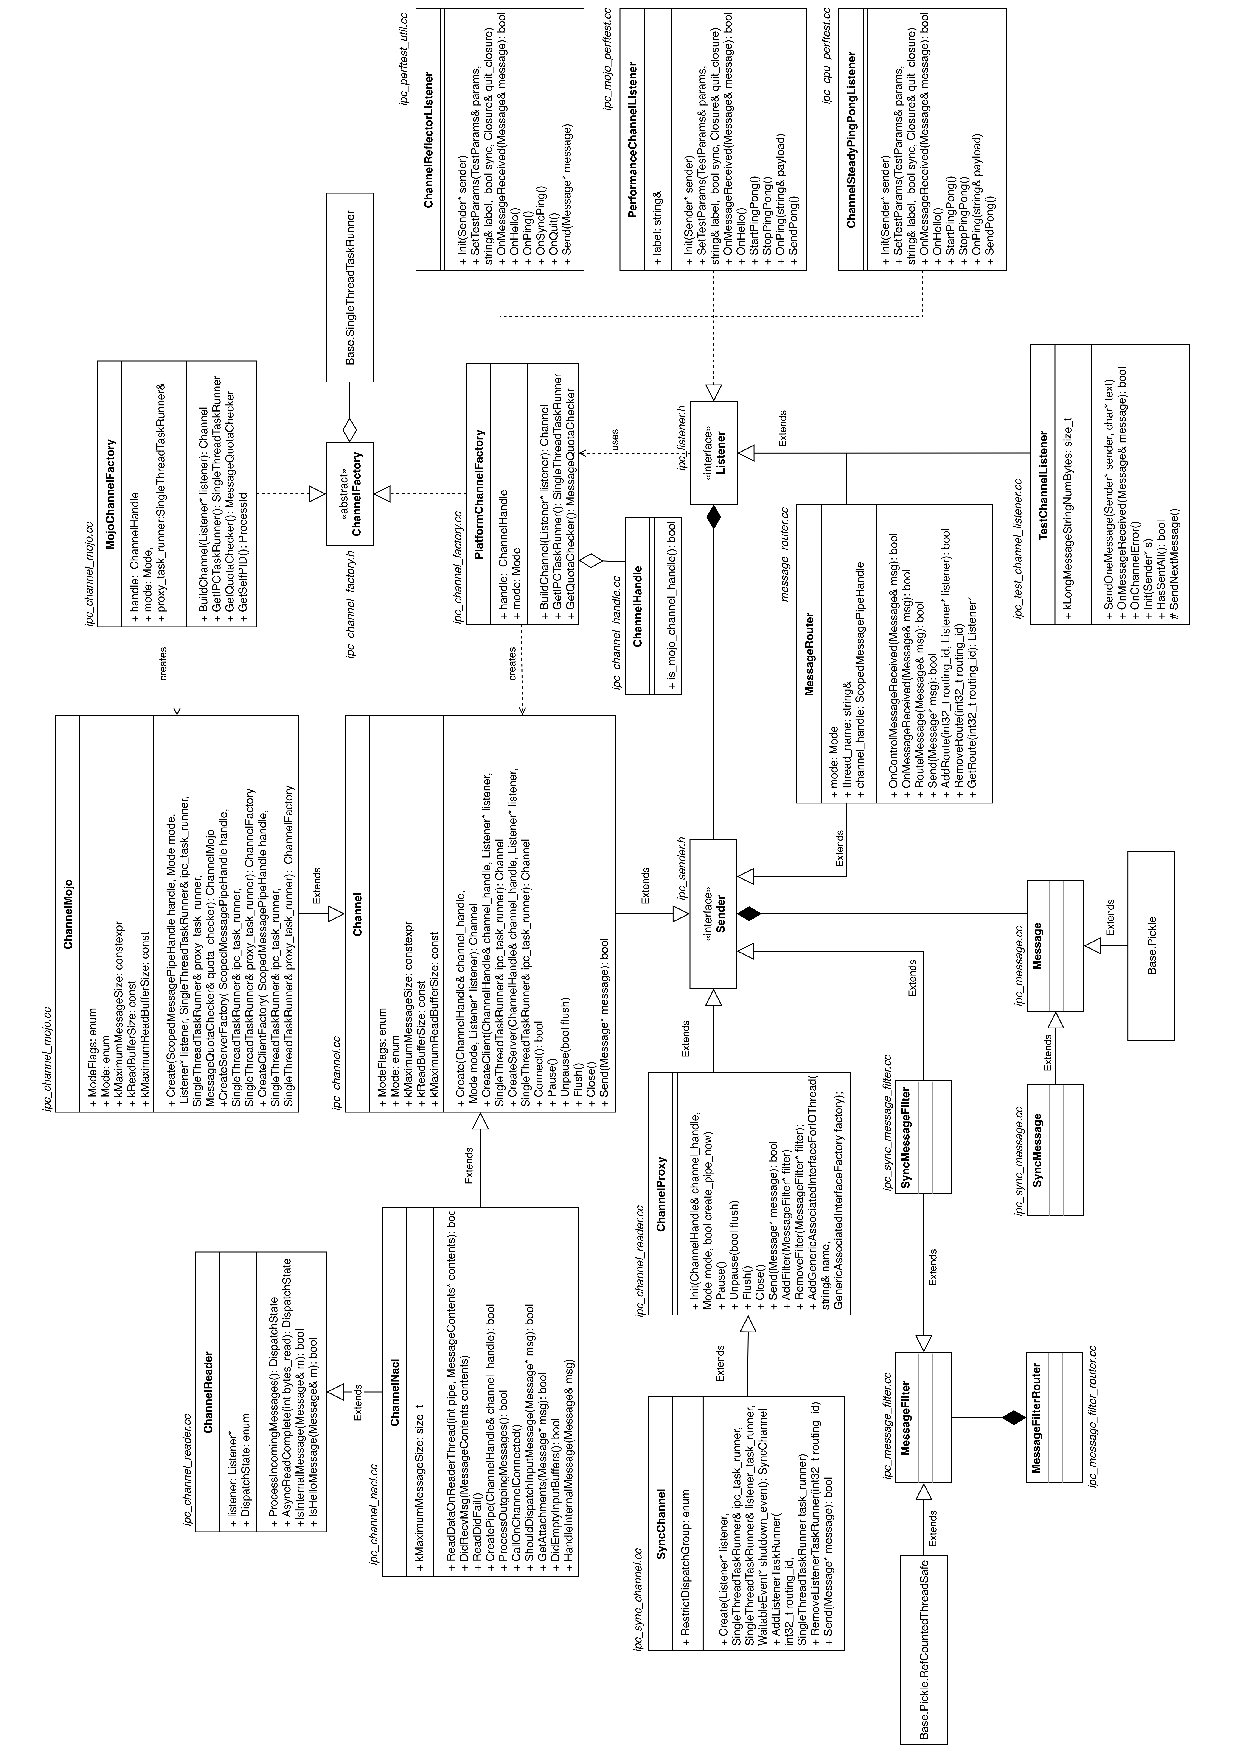
\includepdf[pages=1, fitpaper]{img/design.pdf}
\end{landscape}

\end{document}

